% =====================================================================
% NeuroAI 2.0 Workshop @ AAAI-27 -- LONG PAPER (8 pages + refs + supplementary; archival, PMLR)
% Template: AAAI-27 Author Kit (AuthorKit27, TemplateVersion 2027.1),
%           AnonymousSubmission2027.tex. Double-blind.
% Main content (Abstract..Discussion) must fit in 8 pages.
% References and Supplementary (after references) do not count.
% See README.md for compile command and the formatting checklist.
% =====================================================================
\documentclass[letterpaper]{article} % DO NOT CHANGE THIS
\usepackage[submission]{aaai2027}  % DO NOT CHANGE THIS
% Fonts are loaded by aaai2027.sty. DO NOT add times/helvet/courier/lmodern/any font package.
\usepackage[hyphens]{url}  % DO NOT CHANGE THIS
\usepackage{graphicx} % DO NOT CHANGE THIS
\urlstyle{rm} % DO NOT CHANGE THIS
\def\UrlFont{\rm}  % DO NOT CHANGE THIS
\usepackage{natbib}  % DO NOT CHANGE THIS AND DO NOT ADD ANY OPTIONS TO IT
\usepackage{caption} % DO NOT CHANGE THIS AND DO NOT ADD ANY OPTIONS TO IT
\frenchspacing  % DO NOT CHANGE THIS

% Allowed extras
\usepackage{booktabs}   % tables (recommended by the kit)
\usepackage{amsmath}    % math
\usepackage{amssymb}

% Keep the \pdfinfo exactly as in the kit (no /Title or /Author for anonymity).
\pdfinfo{
/TemplateVersion (2027.1)
}

% DISALLOWED PACKAGES (from the kit): authblk, babel, balance, CJK, epsf, epsfig,
% euler, float, flushend, fullpage, geometry, graphics, hyperref, indentfirst,
% layout, lmodern, multicol, nameref, navigator, pdfcomment, pgfplots, psfig,
% pstricks, savetrees, setspace, stfloats, t1enc, tabu, times, titlesec,
% tocbibind, ulem, wrapfig (or anything that embeds links).
% DISALLOWED COMMANDS: \nocopyright, \addtolength, \balance, \baselinestretch,
% \linespread, \clearpage, \newpage, \pagebreak, \break, \columnsep, \pagestyle,
% \setlength (except \setlength{\tabcolsep}), \textheight, \topmargin, \tiny,
% \abovecaption/\belowcaption, \abovedisplay/\belowdisplay, \float, \clip, \trim,
% \resizebox on tables, negative \vspace/\vskip near captions/floats/headings/refs.

\setcounter{secnumdepth}{0} % unnumbered sections (kit default)

% Simple in-text TODO marker. Remove all uses before submission (grep TODO).
\newcommand{\todo}[1]{\textbf{[TODO: #1]}}
\newcommand{\tbd}{\textbf{??}}
\newcommand{\devnote}{\textbf{[DRAFT: development episodes (16) and four models; replace with held-out results]}} % result cell to fill; see discussion/tables_fill_guide.md
% Placeholder box for figures not yet generated (remove when real PDFs exist).
\newcommand{\figplaceholder}[2]{\fbox{\parbox[c][#2][c]{0.95\linewidth}{\centering\small Figure placeholder: #1}}}

% Title in mixed (title) case, per AAAI. Neutral working title; final wording only after held-out results.
\title{Learning Whom to Trust from Feedback: How History Format Shapes\\In-Context Learning in Vision-Language Models}
% Anonymous author block (double-blind). Do not change.
\author{
    Anonymous Submission
}
\affiliations{
}

\begin{document}

\maketitle

% =====================================================================
% TERMINOLOGY (from research/volatile_trust/discussion/paper_conventions.md; use consistently)
%  advisor / advice-taking (judge--advisor system, Yaniv)    NOT "reporter trust learning"
%  advisor accuracy / reliability                           NOT "source fidelity score"
%  raw history / summarized history (Krishnamurthy et al. 2024)
%  D = description condition = described accuracy ("80% correct") ; A = raw feedback history ; C = summarized history (counts; NOT lossless, NOT a description)
%  description--history (DH) gap (Ge et al. 2026) ; description--experience gap (Hertwig et al. 2004)
%  correctness-only history (our condition B; define on first use)
%  positive recency (copying the last outcome)              NOT "outcome perseveration", NOT "hot hand"
%  CPT regressor: follow the advisor correct on the previous trial (Behrens et al. 2008, Fig. 1e)
%  integration kernel (Lau & Glimcher 2005; Keung et al. 2020) ; x: "Trials in the past", y: "Regression weight (log-odds)"
%  volatility, change-point, hazard rate (Behrens 2007; Nassar 2010; Adams & MacKay 2007)
%  cover story (our scenarios) ; counterbalanced copy (our "twins") ; control conditions (our positive controls)
%  frozen model, in-context ; Psych-101 replay: "conditioned on previously executed behavior" (Centaur)
%  equivalence test (TOST) with smallest effect size of interest = 2 pp
%  95% bootstrap CI over episode pairs (state in every caption)
% =====================================================================

\begin{abstract}
% ~170 words: theme -> question -> approach -> 3 findings -> meaning. Final numbers from held-out only.
Learning whom to trust when an advisor's accuracy changes is a classic test of context-dependent learning in people. We adapt a human advice-taking task to ask whether vision-language models (VLMs), without parameter updates, learn advisor accuracy in context from trial-by-trial feedback, and how this depends on the format of the history. The same history is given raw (both reports and the outcome), as a record of who was correct on each trial, or as counts of correct trials. On 48 held-out episodes, four of five open-weight VLMs answering directly chose at or below chance from raw histories and tended to repeat the previous outcome. A record of who was correct raised accuracy by 8--16 percentage points, to the level of the counts, whereas appending the same record to the raw history helped little; masking parts of the history showed that the visible outcome label drives the repetition. The effect depends on the system and the layout: two proprietary reasoning models, tested on a subset, had similar observed raw-history accuracy to a Bayesian volatility learner (.63), and a compact one-line layout narrowed the gap in two open models. In a changing bandit from Psych-101, a dataset of human choices, participants' estimated forgetting increased with change frequency, while model estimates changed little when replaying participants' histories. The task and analysis code will be released upon acceptance.
\end{abstract}

% \begin{links}  % camera-ready only: public GitHub code link (not in the review version)
%     \link{Code}{https://github.com/XXXX}
% \end{links}

\section{Introduction}
\begin{figure*}[t]
  \centering
  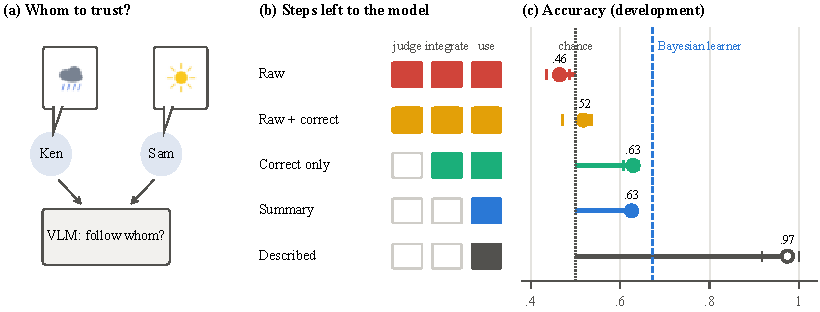
\includegraphics[width=\textwidth]{figures/fig_teaser.pdf}
  \caption{Replacing raw feedback with correctness-only histories improves prediction accuracy. (a) Predictions use past history and current reports; the current outcome is revealed afterwards and enters the next trial's history. (b) Prompt excerpts show the same past trial in three history formats, supplied in separate queries. (c) Equal-weight mean accuracies over five open models on 48 held-out test episode pairs with text reports. A pair comprises an episode and its counterbalanced copy, with advisor names and answer labels swapped. The open diamond marks all-trial summaries; the dashed line marks 50\% chance. Model-level results and 95\% bootstrap confidence intervals (CIs) appear in Fig.~\ref{fig:gap}a.}
  \label{fig:teaser}
\end{figure*}

People learn whom to trust from feedback. When two advisors disagree and the outcome is revealed afterwards, people keep track of how often each advisor was right, and they update this estimate faster when the advisor's accuracy is volatile \citep{behrens2008associative}; advisor reputations form quickly from a track record \citep{yaniv2000advice,bonaccio2006advice}. Because this advice-taking task comes from human neuroscience, a model can be tested with the same design and analysed with the same computational models. We use a simplified variant without human data; our direct comparison with people uses a second task with published human choices.

Agents built on large language models (LLMs) and vision-language models (VLMs) face the same problem when they combine tool outputs, retrieved documents or messages from other agents whose reliability can change. Prior work asked whether LLMs weight sources by reliability when it is fixed \citep{ashkinaze2026information}, flips once \citep{zhou2026epistemic} or breaks after scripted failures \citep{chen2026trust}, and proposed memories that track reliability outside the model \citep{feng2026sigmamem}. Whether a model without fine-tuning can learn a changing, non-stationary accuracy by in-context learning from trial-by-trial feedback, and which part of the computation fails if it cannot, is open. This is context-dependent learning without parameter updates: each query receives the accumulated history, and the model's choices do not change later feedback.

The format of past evidence is known to matter. LLMs choose differently when outcome probabilities are described than when they are experienced \citep{ge2026dhgap}, explore well in bandits only with summarized histories \citep{krishnamurthy2024explore}, and integrate evidence with strong recency \citep{xue2026counting}. These tasks do not require deriving advisor correctness by comparing conflicting reports with observed outcomes.

Learning whom to trust involves three computations: (i) judging which advisor was correct on each trial, (ii) integrating these judgments across trials, and (iii) using the estimate. Five VLMs receive the same history in formats that state these results to different degrees (Fig.~\ref{fig:teaser}b), plus a condition describing advisor accuracy. Formats also change length and salience; we test which representations support good choices without assuming separable internal stages. Our contributions are:
\begin{itemize}
  \item[$\bullet$] An advice-taking evaluation adapted from human neuroscience, with text and image reports; task generation, prompts and analysis code will be released upon acceptance.
  \item[$\bullet$] Across five open VLMs answering directly, correctness-only histories remove most of the summary--raw gap, whereas a visible outcome label elicits repetition of the previous outcome, as predicted before a held-out masking test.
  \item[$\bullet$] A boundary condition: two proprietary reasoning models have similar observed raw-history accuracy to a Bayesian learner, so the format effect depends on the system.
  \item[$\bullet$] A comparison of models with people in a second task, the changing bandit of Psych-101.
\end{itemize}

\section{Related Work}
\paragraph{Cognitive evaluation of LLMs.} Treating a language model as a participant in a psychological experiment is now a common way to characterize its behavior \citep{binz2023using}. CogBench turns such experiments into behavioral metrics \citep{codaforno2024cogbench}, and Centaur is a model fine-tuned to predict trial-by-trial human choices in Psych-101 \citep{binz2025foundation}. Fits of reinforcement-learning models to in-context behavior in bandits have found asymmetric or biased updating and rigid or greedy choice \citep{schubert2024incontext,hayes2024biased,wang2026rigidity,schmied2025greedy}, and reversal-learning schedules have been compared across LLMs \citep{wang2026comparative,li2025reflectionbench}. The bandit and reversal-learning evaluations focus on learning option values rather than extracting advisor correctness from report--outcome pairs.

\paragraph{Description, experience and history summaries.} The description--experience gap \citep{hertwig2004decisions,wulff2018metaanalytic} has an LLM counterpart in the description--history gap of \citet{ge2026dhgap}. \citet{krishnamurthy2024explore} contrasted raw and summarized histories in bandits, and \citet{xue2026counting} traced integration kernels (weights on evidence at different lags) in a counting task. LLMs also update roughly as Bayesian observers when the observed sequence is itself what they predict \citep{gupta2025coinflips,zhang2025discounted}. Our summarized history is computed from the same history the model would otherwise see; it discards trial order and is not a description. Source-history interventions also distinguish recognizing reliability from allowing it to influence a decision \citep{zhang2026evidence}. We extend this question to repeated reversals and test which components of trial-by-trial feedback trigger outcome repetition.

\paragraph{Volatility and multimodal reports.} Our task follows the social-learning paradigm of \citet{behrens2008associative}. Normative accounts of learning under volatility include hierarchical Bayesian and change-point models \citep{behrens2007learning,nassar2010approximately,nassar2012rational,mathys2011bayesian,piray2021model,piray2024computational,soltani2019adaptive}, and social and individual learning can be arbitrated separately \citep{diaconescu2020neural}. For image reports, performance depends on modality even when content is isomorphic \citep{fu2024isobench}, multi-image inputs show position biases \citep{tian2025position}, and VLMs have difficulty binding features to objects \citep{campbell2024binding}.

\section{Task and Methods}
\paragraph{Advice-taking task.} On each trial, two advisors give conflicting binary reports (for example, rain and dry), the model predicts the outcome, which amounts to choosing whom to follow, and the outcome is then revealed. An episode has 80 trials. Advisor A is correct with probability 0.8 in a stable phase of 40 trials; in a volatile phase of 40 trials its accuracy alternates between 0.8 and 0.2 every 10 trials (each switch is a reversal), following \citet{behrens2008associative} (comparison in Appendix~B). Half of the episodes start with each phase. Outcome sequences are pre-generated, so the model's choices do not change the history, within each 10-trial block A's realized accuracy equals the scheduled value, and each outcome label appears five times. The instructions say that an advisor's accuracy may change but give no rate.

Each episode is shown with a pet cover story, in which reporters say whether a hidden animal is a cat or a dog, and with one of six non-pet cover stories (colors, weather, stocks, sports, medical tests, news; Appendix~A). Current reports are given as text or as an image: a drawn icon for the non-pet cover stories and a photograph \citep{parkhi2012cats} for the pet cover story; with text reports, both cover stories are text only. Every episode has a counterbalanced copy in which advisor names and answer labels are swapped while outcomes are identical; averaging over the two cancels name and label biases. The 16 development episodes were used to choose settings; 48 separate episodes form the held-out test set. A robustness set has 24 episodes with independent outcomes and irregular reversals.

\paragraph{History formats.} Before trial $t$, the model sees trials $1,\dots,t-1$ in one format (examples in Fig.~\ref{fig:teaser}b; full prompts in Appendix~A). The \emph{raw history} lists both reports and the outcome (``Day 3: Ken forecasts rain; Sam forecasts dry. Actual weather: rain.''). \emph{Raw + correctness} appends ``(Ken was correct; Sam was wrong.)'' to each trial. \emph{Correctness only} keeps only that statement, stating the result of step (i). The \emph{summary} gives each advisor's number of correct trials so far, stating the result of steps (i) and (ii); it discards trial order. Further summaries count over the last $K$ trials or since a change point inferred by Bayesian online change-point detection (BOCPD; \citealt{adams2007bocpd}; Appendix~E), and a chart draws who was correct as an image.

\paragraph{Control conditions.} On development episodes, control items give the answer more directly: \emph{described accuracy} (``Ken was correct on 80\% of past days''), described counts, short and long easy histories in raw and correctness-only form, and a single raw trial on which the model names who was correct (step (i) alone).

\paragraph{Models and readout.} We test five open-weight VLMs without fine-tuning, four of them built on Qwen3 language models: Qwen3-VL 8B and 32B \citep{bai2025qwen3vl}, InternVL3.5 8B and 38B, which use a Qwen3 language model \citep{wang2025internvl35}, and Gemma-3-27B \citep{gemmateam2025gemma3}. The open models are prompted to answer directly with one word. Two proprietary reasoning models are tested through application programming interfaces (APIs) on a subset; their choice is read from the generated answer (Appendix~K). The readout is the choice probability $y_t$ for advisor A's report, from the logits (unnormalized output scores) of the two answer words at the first generated token, normalized over these two words; it is not a belief. For four models nearly all probability mass fell on the two answer words; Gemma-3-27B often began a sentence instead when given a summary (Appendix~K).

\paragraph{Measures and analysis.} Accuracy is the proportion of trials ($t\ge2$) on which the higher-logit answer is correct, after averaging label-aligned logits over the counterbalanced copies; exact ties receive half credit and chance is 0.5. To describe behavior we fit a logistic regression of $y_t$ on which advisor was correct $k$ trials back, whose weights over $k$ form an integration kernel \citep[cf.][]{xue2026counting}, plus a regressor for repeating the previous outcome, and compute agreement (Cohen's $\kappa$) with simple strategies. We also fit learning models (a constant bias, delta rules, counts over all or recent trials, change-point and volatility learners) to each model's choice probabilities and compare them by leave-one-episode-out cross-validation (Appendix~F). As a computational reference we run the Bayesian volatility learner of \citet{behrens2007learning,behrens2008associative} on the same episodes; it receives who was correct on each trial, and it is optimal under its own assumption of independent trials, not under our block schedule. The unit of analysis is the episode pair (an episode and its counterbalanced copy), and uncertainty is reported as 95\% confidence intervals (CIs) from a bootstrap over episode pairs (10{,}000 resamples). These CIs are pointwise: they are not adjusted for simultaneous coverage across estimates. The primary test, fixed before held-out evaluation, is the summary$-$raw accuracy difference per model (Wilcoxon signed-rank test, Holm-corrected across models; required in both language-model families). Secondary tests and all other details are in Appendix~C.

\paragraph{Human comparison.} We replay the changing-bandit task of \citet{xiong2023neural} from Psych-101: 30 participants, three change probabilities (hazard rates, $h$) and 100 trials per game. The hazard rate is the probability that a machine's payoff changes on each trial. Models see each participant's preceding choices and payoffs, with $h$ hidden or stated. We fit the original model-free learner to human choices and sampled model choices. Its forgetting rate $\phi$ moves the unchosen machine's estimated value toward the midpoint of the payoff range; we compare slopes of $\phi$ on $h$, paired by participant (Appendix~I).

\section{Results}
\begin{figure*}[t]\centering
  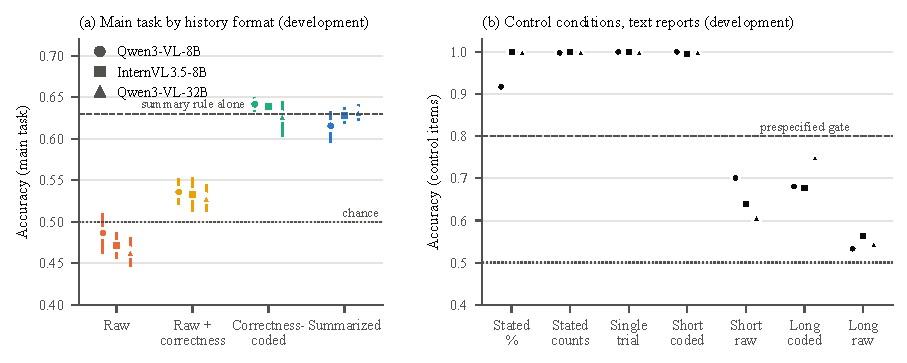
\includegraphics[width=\textwidth]{figures/fig_gap.pdf}
  \caption{History-format effects depend on the system. (a) Separate panels show each open model across four history formats on 48 held-out episode pairs, after aligning and averaging logits across counterbalanced copies. (b) Seven systems on matched trials (24 episode pairs, every fourth trial), with one panel per history format and each copy scored separately; open-model choices use candidate logits, API choices generated answers (valid answers only). Colours denote history formats; models are labelled directly. Bars show 95\% bootstrap CIs from resampling episode pairs; reference lines mark 50\% chance. The comparison does not isolate reasoning from other system differences.}
  \label{fig:gap}
\end{figure*}

\begin{table*}[t]\centering\small
  \setlength{\tabcolsep}{6pt}
  \begin{tabular}{l rrrr r c}
    \toprule
    Model & Raw & Raw+corr. & Corr.\ only & Summary & Summary$-$raw [95\% CI] & $p_\text{Holm}$ \\
    \midrule
    \multicolumn{7}{l}{\textit{Full test set: 48 episode pairs; copies combined before scoring}} \\
    Qwen3-VL-8B & 48.6 & 51.7 & 61.9 & 62.1 & +13.4 [12.2, 14.6] & $<$.001 \\
    InternVL3.5-8B & 47.9 & 50.8 & 63.6 & 63.5 & +15.6 [14.5, 16.7] & $<$.001 \\
    Gemma-3-27B & 47.0 & 49.8 & 60.2 & 61.7 & +14.7 [13.2, 16.3] & $<$.001 \\
    Qwen3-VL-32B & 46.8 & 52.2 & 62.8 & 63.1 & +16.4 [15.0, 17.7] & $<$.001 \\
    InternVL3.5-38B & 54.9 & 56.0 & 62.5 & 63.3 & +8.4 [7.4, 9.4] & $<$.001 \\
    \midrule
    \multicolumn{7}{l}{\textit{API subset: 24 episode pairs, every fourth trial; copies scored separately}} \\
    GPT-6-Astra & 62.8 & -- & 62.3 & 58.5 & $-$4.3 [$-$8.8, 0.3] & -- \\
    Claude Fable 5.2 & 62.9 & -- & 62.4 & 58.5 & $-$4.4 [$-$8.6, 0.1] & -- \\
    \midrule
    \multicolumn{7}{l}{\textit{Computational references: full set / API subset}} \\
    Bayesian learner & \multicolumn{4}{c}{66.8 / 62.9} & -- & -- \\
    All-trial count & \multicolumn{4}{c}{63.2 / 58.5} & -- & -- \\
    Last-five count & \multicolumn{4}{c}{69.2 / 67.9} & -- & -- \\
    \bottomrule
  \end{tabular}
  \caption{Correctness-only histories raise accuracy in the five open models. Accuracy is in percent; differences and their paired 95\% bootstrap CIs are in percentage points. Full-set scores average the two cover stories after aligning and averaging the counterbalanced logits. API scores use generated answers on a smaller set of trials and are reported separately; Fig.~\ref{fig:gap}b compares all systems on the same trials with per-copy scoring. Raw+corr.: raw history with correctness appended. Primary $p$-values are Holm-corrected across the five open models; complete tests, chart results and controls appear in Appendix~C.}
  \label{tab:main}
\end{table*}

\begin{figure*}[t]\centering
  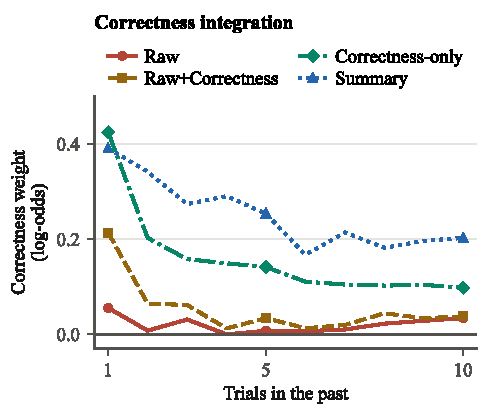
\includegraphics[width=\textwidth]{figures/fig_kernel.pdf}
  \caption{Outcome masking improves accuracy; additional report masking yields further gains. (a) Correctness integration kernels by history format, averaged over the five fixed open models on held-out test episodes; per-model kernels and CIs appear in Fig.~\ref{fig:kernel_models}, and raw-history strategy agreement in Fig.~\ref{fig:strategies}. (b) Rows indicate whether past outcomes are shown or masked; columns indicate whether past advisor reports are shown or masked. Correctness statements remain visible in every condition. Cells show mean accuracy (\%) on 48 held-out episode pairs with text reports, using a common colour scale. Paired changes from raw + correctness and their 95\% bootstrap CIs appear in Fig.~\ref{fig:masking_effects}.}
  \label{fig:kernel}
\end{figure*}

\paragraph{Open models use described accuracy, but not experienced reliability.} With text reports, described accuracy or counts led the models to choose the advisor described as better on 92--100\% of items (a different measure from main-task accuracy), and every model named the correct advisor on a single shown trial (Fig.~\ref{fig:controls}; development episodes). The same information was used much less when it had to be learned. In an easy raw history in which one advisor had been right on every recent trial, models followed that advisor on .60--.79 of items after 10 trials and on .53--.70 after 80. Stating who was correct on each trial raised this to 1.00 for 10 trials, but only to .67--.90 for 80 trials. Judging one trial is therefore not the difficulty; judging many trials is, and long histories remain hard even when this step is done for the model.

\paragraph{Stating who was correct closes the gap; appending it does not.} On held-out episodes, accuracy was .468--.486 with raw histories in four models and .549 [.538, .560] in InternVL3.5-38B, the only model above chance, and .617--.635 with summaries (Fig.~\ref{fig:gap}a; Table~\ref{tab:main}). The summary$-$raw gap was $+.084$ to $+.164$ and significant in every model (Holm-corrected $p<.001$; Table~\ref{tab:tests}), so the primary test held in both language-model families. Scoring each counterbalanced copy separately preserved positive gaps in all five models ($+8.8$ to $+13.9$ points; Appendix~K). A correctness-only history attained .602--.636 accuracy, close to the summarized history, although it still leaves integration to the model. Integration was nonetheless imperfect: this history remained below a count over the last five trials (.692) and lagged after reversals (below). Appending the same statement to the raw history improved accuracy by only 1.1--5.4 percentage points, even though the model then had all the information of the correctness-only history. The raw reports and outcomes therefore do more than add work: they interfere with using the statement next to them, which the next analyses explain. The size of the gap depends on presentation: with a compact one-line record per trial, raw-history accuracy rose to .55--.56 while correctness-only and summarized histories fell, shrinking the gap to 1--3 points in the two 8B models; raw accuracy stayed below the count rule in every layout (development episodes; Appendix~J).

\paragraph{Under raw histories, open models tend to repeat the previous outcome.} The kernel weights on past correctness were near zero, while the weight on repeating the previous outcome was positive in every model (Fig.~\ref{fig:kernel_models}; correctness kernel in Fig.~\ref{fig:kernel}a). Repeating the previous outcome agreed best with the models' choices ($\kappa = .22$--.32 in four models and .13 in InternVL3.5-38B, whose choices also agreed weakly with recent counts; Fig.~\ref{fig:strategies}). The 15-lag kernel describes local sensitivity to recent trials and cannot by itself separate a recency-weighted learner from an all-trial count on this schedule; computational-model comparisons are specified in Appendix~F. \todo{held-out model fits} Because each 10-trial block contains each outcome five times, repeating the previous outcome scores below chance (.445 on held-out episodes), which explains accuracy below .5; on the robustness set, where outcomes are independent, raw-history accuracy was near chance (.507--.520) in four models. When the history stated who was correct, the kernel instead peaked at the most recent trial and decayed over the next few, and the weight on the previous outcome vanished.

\paragraph{Masking identifies the outcome label as a trigger.} We replaced parts of the raw history with correctness by a dash while retaining its layout. Development results motivated predictions for a five-model held-out replication (Appendix~J). On held-out episodes, all predictions written before the run held in all five models: replacing the outcome label helped by 2.7--6.4 points and reduced the weight on the previous outcome from .42--.87 to .08--.23, replacing the reports alone changed accuracy by at most 0.4 points, but once the outcome label was replaced, also replacing the reports added 2.1--5.5 points, and with both replaced accuracy came within 4 points of the correctness-only history (Fig.~\ref{fig:kernel}b; Appendix~J). The visible outcome label drives the repetition; the reports matter once it is removed.

\paragraph{Reliability judgments and choices are weakly aligned.} Asked which advisor was currently more likely to be correct, the models named the scheduled better advisor on .60--.67 of raw-history trials, below always naming the advisor that was better over most of the episode (.75), with little agreement with any rule ($\kappa\le .17$), and their choices followed their own judgment on only 53--69\% of trials ($\kappa\le .12$; Appendix~J). Judgments and choices were weakly aligned.

\paragraph{A computational reference for evidence integration.} The Bayesian volatility learner of \citet{behrens2008associative}, run on the same held-out episodes, made correct choices on .668 [.661, .674] of trials, above the all-trial count rule (.632) and above every open model given raw, correctness-only or all-trial summarized histories (Table~\ref{tab:main}; Appendix~B). It receives who was correct on each trial, so it benchmarks integration separately from reading the history, and it is not human performance. A count over the last five trials, selected on development episodes with the same schedule, scored higher (.692), and only models given such a recent-trial summary, computed outside the model, reached the learner (.666--.691; Appendix~E). With 80 trials, even this learner's learning rate rises only slightly in the volatile phase, too little to test volatility adaptation here (Appendix~F).

\paragraph{A summary passes on its rule, including its lag.} Given all-trial counts, models chose the advisor with more correct trials on 94--100\% of non-tied trials, and four of five were equivalent to the rule alone within $\pm$2 points (Gemma-3-27B: $-.014$, $p_\text{Holm}=.053$; Table~\ref{tab:tests}). A model that follows a summary therefore inherits the rule's response to change. The all-trial count lags behind every reversal (Appendix~A, Fig.~\ref{fig:task}b): after a reversal, the mean probability of following the currently better advisor stayed below .5 early in the block with either this summary or the correctness-only history, then rose above .5; with raw histories it stayed near .50 (Fig.~\ref{fig:curves}). Summaries over the last five trials or since a change point inferred by BOCPD were followed as faithfully (agreement .94--1.00; equivalent to the rule in five of five models for the change point and three of five for the window), and the mean following probability exceeded .5 two to three trials after a reversal; overall accuracy was .666--.691, 4--6 points above the all-trial summary and 4--8 points above the correctness-only history (Appendix~E). How fast an agent built this way adapts to a volatile source is therefore set by the rule outside the model.

\paragraph{Proprietary reasoning models learn from raw histories.} On a held-out subset (24 episode pairs, every fourth trial; Appendix~K), Claude Fable 5.2 made correct choices on .629 [.592, .665] of trials with raw histories, .624 with the correctness-only history and .585 [.544, .627] with the all-trial summary (summary$-$raw $-.044$ [$-.086$, .001]); GPT-6-Astra gave nearly identical values (.628, .623 and .585; $-.043$ [$-.088$, .003]). On the same trials the open models reached .446--.529 with raw histories, the Bayesian learner .629, and the count rules .585 (all trials) and .679 (last five). Correctness labels did not increase mean accuracy for these models, and the all-trial summary was numerically lower than the raw history, at the level of its rule. These models reason before answering (visible reasoning in 77\% of Fable's raw answers) and also differ from the open models in scale, training and readout, so the comparison sets a boundary on the format effect rather than isolating an effect of reasoning. Their raw-history choices tracked the advisors rather than a shortcut (exploratory; Appendix~K): they agreed with the Bayesian learner ($\kappa=.78$--.87) and the last-five count (.77--.79), not with repeating the previous outcome ($\kappa\approx 0$) or with the outcome quota (.07--.10), a rule that would score .702 on these trials; where the quota and the learner disagreed they followed the learner on 91--96\% of trials, and after a reversal they followed the newly better advisor on .06--.09 of trials in the first three trials of the reversed block, rising to .94--.99 in trials 8--10. Given the all-trial summary, both chose exactly as the count rule ($\kappa=1.00$). Scored per copy in the same way, the open models were less accurate than with the averaged readout (raw .467--.503, correctness-only .523--.589, summary .533--.590), because single copies keep the name and label biases that averaging cancels. \todo{reasoning checkpoint}

\paragraph{Image reports add context-dependent costs (exploratory).} Models named a single report image almost perfectly, yet with described accuracy and image reports they followed the better advisor on only .59--.84 of items, in four models least when the advisor's name was given only after the image (Appendix~G). Accuracy was mostly higher when the name was printed on the image or both reports were shown in one labelled image, although each panel was read correctly. On held-out episodes much of the cost came from choosing the first-listed image: with the correctness-only history, four models chose the first-listed report on 79--92\% of trials with images but 44--54\% with text, and their accuracy fell to .11--.24 when the correct report was listed second (Appendix~J). With the correctness-only history, image reports lowered held-out accuracy by 7--10 points compared with text reports (.523--.552). Models could not read single cells of the correctness chart reliably (.61--.71), so chart histories are not interpreted.

\paragraph{Humans and models in the changing bandit.} In the changing bandit of Psych-101, a normative learner forgets the unchosen option faster when the hazard rate is higher, and participants did (median forgetting rate .079 at $h=0.1$, .255 at $h=0.4$; Appendix~I). Unlike the advice task, this task varies volatility across games. Models replayed participants' histories; participants had also played earlier games, so the comparison is descriptive. A simulation of the whole pipeline gave a false-positive rate of 6\% but only about half the power for a difference as large as the human effect (Appendix~I), so a null result would not show similarity. Model estimates varied less with hazard rate. Their median forgetting rate was at most .051 at every hazard rate, and the per-participant slope on hazard rate was $-0.01$ to $0.04$, against 0.47 for the participants (Fig.~\ref{fig:human}, Table~\ref{tab:psych}). All five paired differences were negative ($-0.48$ to $-0.60$), four at an uncorrected $p<.05$ ($p=.011$--.070), none after Holm correction across the five models. Stating the hazard rate, which matches what participants were told, did not produce a clear change (slopes $-0.04$ to $0.16$). Forgetting rates near zero are estimated at the boundary of the parameter range, so we checked this in a separate regression: the models' choices did depend on the machines' last observed values (positive weight for 77--100\% of participant histories), but whereas participants weighted a value difference less when the older value was stale (seen four or more trials earlier; stale/fresh weight ratio .58--.86), the models weighted stale differences as much or more (.95--2.07; Appendix~I). This exploratory contrast does not establish a hazard-dependent adaptation deficit: the human discounting estimate did not increase with hazard rate, and replay differs from acting in the task.

\begin{figure}[t]\centering
  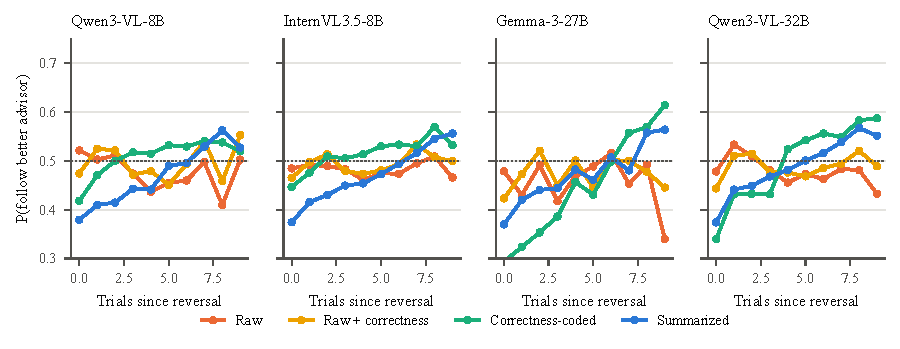
\includegraphics[width=\columnwidth]{figures/fig_curves.pdf}
  \caption{Recent-trial summaries recover higher following probabilities sooner after a reversal. Curves are mean choice probabilities over the five fixed models on held-out episodes, with line styles and colours identifying history formats. The dotted horizontal line marks .5; pointwise uncertainty is not shown. Per-model curves appear in Fig.~\ref{fig:curves_models}.}
  \label{fig:curves}
\end{figure}
\begin{figure*}[t]\centering
  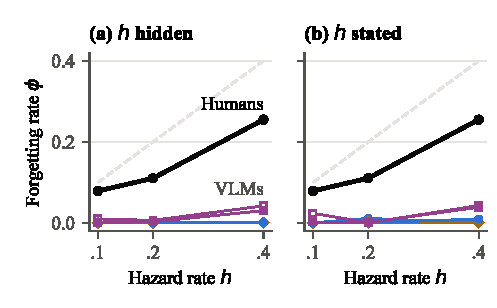
\includegraphics[width=\textwidth]{figures/fig_human.pdf}
  \caption{Human--model forgetting-rate comparisons remain descriptive. (a,b) Median fitted forgetting rate $\phi$ by hazard rate, with $h$ hidden or stated for the model; humans were told $h$ in both panels. Model estimates are medians over 20 fits to sampled binary-choice sequences. (c) Paired model-minus-human slope differences for the same 30 participant histories, with unadjusted 95\% CIs from resampling participants. Solid and dashed intervals mark hidden and stated $h$; marker shape and fill identify the five models. None of the five hidden-$h$ comparisons is significant after Holm correction. The simulation study shows limited power and an upward bias (Appendix~I); these results do not establish equivalence.}
  \label{fig:human}
\end{figure*}
% FILL: analyze_main.py held-out JSON -> cells / gaps (domain=all); D from analyze_controls.py (explicit_rel hard_acc).

% FILL: analyze_main.py held-out JSON -> gaps[primary=True] (mean, ci95, p_wilcoxon, p_holm) and
%       tost[rule=window_counts, domain=all] for C in {sum_all, sum_cp, sum_window:K*} (families/secondary).

\section{Discussion}
Across five open VLMs answering directly, how the history was represented decided whether advisor accuracy was learned. The models used described accuracy and followed a summary as faithfully as its rule, yet four of five chose at or below chance from the raw record. A record of who was correct removed most of the gap, the same record appended to the raw history helped little, and masking showed that the visible outcome label elicited repetition of the previous outcome. This suggests a refinement of the description--history gap \citep{ge2026dhgap}: in these models, experience is used poorly not mainly because it must be integrated, but because the raw record invites a competing response before the relevant observation, who was correct, is extracted. Our manipulations change what the history states, not internal stages, so they do not localize a failed internal computation. The effect is also not universal: two proprietary reasoning models had similar observed raw-history accuracy to the Bayesian learner, with no increase in mean accuracy from correctness labels. In the human study, who was correct is the observation from which a prediction error about the advisor is computed \citep{behrens2008associative}; our interventions change how this observation is represented and make no claim about an internal error signal or its neural implementation.

\paragraph{Implications for NeuroAI.} For building agents, an explicit record of which source was correct, and an integration rule outside the model, help models that struggle with raw histories: with a last-five-trial summary, mean following probability exceeded .5 three trials after a reversal; with all-trial counts it crossed .5 six trials after the reversal and reached only .56 at the end of the ten-trial window (Fig.~\ref{fig:curves}). For models that already use raw histories, a lossy summary can instead remove information. For neuroscience, the format manipulation offers a way to test candidate models of advice taking against the behavioural signatures used for people; the open VLMs tested here do not yet show those signatures. These parallels are computational. In the changing bandit, participants' estimated forgetting increased with hazard rate, while model estimates varied less even when told the rate; the paired differences were not significant after correction. The two tasks probe complementary demands of adaptive inference, extracting source-relevant evidence and discounting stale information, and we do not assume that they share one mechanism. \todo{reasoning checkpoint, one sentence}

\paragraph{Limitations.} The task simplifies \citet{behrens2008associative}: two perfectly opposed advisors, no separate reward stream, and no human data on this variant. It is binary, with fixed outcome quotas, which allow shortcuts and make past outcome labels informative about future ones, information that the correctness-only history removes; we therefore repeat the primary test on episodes with independent outcomes, where the gap was about half as large ($+.036$ to $+.083$) but significant in every model (Appendix~J). Eighty-trial episodes are too short to test volatility-dependent learning rates, which we test only in the changing bandit, where the human comparison is descriptive: participants were told the hazard rate and had played earlier games, and the test has about half the power for an effect of the human size. The summary discards trial order, and the size of the summary--raw gap depends on the history's layout (Appendix~J). The open models (up to 38B, four of five built on Qwen3) were prompted to answer directly; the proprietary models were tested on a subset and differ in several respects at once. Images enter only as current reports. The analysis plan was fixed by a timestamped commit; deviations are listed in Appendix~K.

% ---------------------------------------------------------------------
% \section*{Ethical Statement}  % optional
% \section*{Acknowledgments}    % omit for review
% ---------------------------------------------------------------------

\bibliography{refs}

\appendix
\section{Supplementary Material}
% No page limit (workshop CFP). Order follows the main text.
\subsection{A. Prompts and Cover Stories}            % exact templates for all 7 cover stories, A/B/B'/C/D, icons
Every prompt has four parts: instructions naming the two advisors and the cover story, the history in one of the formats of the main text, the current reports, and the question. Prompts are passed through each model's chat template as a single user message. For InternVL3.5 the template adds the model's default system message (in Chinese) and the suffix ``Answer the question using a single word or phrase.'' All answer words are single tokens in every tokenizer used.

\paragraph{Task details.} Each episode is shown with two cover stories that share the same outcome sequence: a pet cover story, in which reporters say whether a hidden animal is a cat or a dog, and one of six other cover stories (colors, weather forecasts, stock predictions, sports predictions, medical readings, news claims), assigned in blocks so that cover story is crossed with phase order (Fig.~\ref{fig:task}). Cover stories change only the wording, the answer words and the report images; all outcome sequences are synthetic. Current reports are text or an image: a programmatically drawn icon without text for the non-pet cover stories, and a photograph from the Oxford-IIIT Pet dataset \citep{parkhi2012cats} for the pet cover story (with text reports the pet cover story is text only, like the others). Both advisors' correctness is revealed on every trial (full feedback). In the counterbalanced copy, advisor names, answer labels and the order in which the instructions introduce the advisors are swapped while outcomes and images are identical; within each trial the two reports are listed in random order. The instructions say that an advisor's accuracy may change over time but give no rate. The held-out set has eight episodes per non-pet cover story.

\begin{figure*}[h]
  \centering
  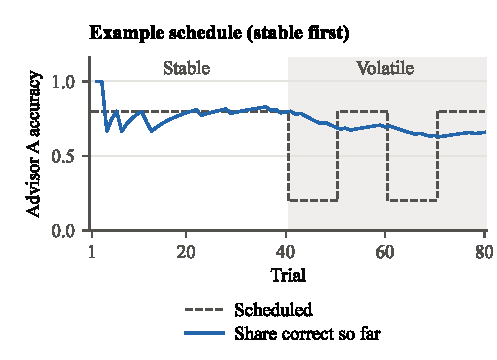
\includegraphics[width=\textwidth]{figures/fig_task.pdf}
  \caption{Task and history formats. (a) One trial in the weather cover story. (b) Scheduled accuracy of advisor A in a stable-first episode (dashed) and the share of past trials on which A was correct, which the all-trial summary reports (solid): it tracks the stable phase but lags behind every reversal. (c) History formats and the processing steps each leaves to the model: (i) outcome evaluation, (ii) integration across trials, (iii) use.}
  \label{fig:task}
\end{figure*}

Table~\ref{tab:cover} lists the cover stories. The examples below are rendered by the experiment code from the fixed episode files; line breaks are as in the prompt and \emph{[image]} marks where an image is inserted.

\begin{table}[h]
  \centering
  \small
  \setlength{\tabcolsep}{3pt}
  \begin{tabular}{llll}
    \toprule
    Cover story & Advisors & Answers & Report image \\
    \midrule
    color & reporters & red/blue & color patch \\
    weather & forecasters & rain/dry & cloud, sun \\
    stock & analysts & up/down & trend arrow \\
    sports & commentators & win/lose & happy/sad face \\
    medical & doctors & positive/negative & plus/minus \\
    news & news sources & true/false & tick, cross \\
    pet & reporters & cat/dog & photograph \\
    \bottomrule
  \end{tabular}
  \caption{Cover stories with the selected icon set (v3.1). Trials are called trials (color, pet), days, weeks, games, cases or stories. Icons are drawn by code and contain no answer words. Appendix~G shows the original and selected medical and sports icons and identifies results obtained with the original set.}
  \label{tab:cover}
\end{table}

\paragraph{Example 1: raw history, weather, held-out episode, trial 6.}
\begin{quote}\small
You are observing a sequence of days. On every day, two weather forecasters, Tim and Joe, give conflicting forecasts for the day's weather (rain or dry). After each day, the actual weather is observed. A forecaster's accuracy may change over time.\\
Past days:\\
Day 1: Joe forecasts rain; Tim forecasts dry. Actual weather: dry.\\
Day 2: Tim forecasts rain; Joe forecasts dry. Actual weather: rain.\\
Day 3: Tim forecasts rain; Joe forecasts dry. Actual weather: rain.\\
Day 4: Joe forecasts rain; Tim forecasts dry. Actual weather: dry.\\
Day 5: Tim forecasts rain; Joe forecasts dry. Actual weather: rain.\\
Current day 6 (actual weather not yet observed):\\
Joe forecasts: dry\\
Tim forecasts: rain\\
Predict the actual weather on the current day. Answer with exactly one lowercase word: rain or dry.
\end{quote}
The other formats change only the history lines. In the raw history with correctness, day 1 reads ``Day 1: Joe forecasts rain; Tim forecasts dry. Actual weather: dry. (Joe was wrong; Tim was correct.)''. In the correctness-only history it reads ``Day 1: Joe was wrong; Tim was correct.''. In the summarized history the five history lines and the ``Past days:'' line are replaced by ``Summary of all 5 past days: Joe was correct 0 times; Tim was correct 5 times.''. In the correctness chart they are replaced by ``Past days 1-5 are summarized in this chart (days run left to right in four lines of 20; for each day, a green square means that forecaster was correct, a gray square means that forecaster was wrong, an empty square means not yet played):'' followed by the chart (448 px; one row per advisor in each line). In the judgment readout the current reports and question are replaced by ``Before day 6: which forecaster is currently more likely to be correct? Answer with exactly one name: Joe or Tim.''.

\paragraph{Example 2: described accuracy, weather, development episode.}
\begin{quote}\small
You are observing a sequence of days. On every day, two weather forecasters, Jim and Ken, give conflicting forecasts for the day's weather (rain or dry). After each day, the actual weather is observed. A forecaster's accuracy may change over time.\\
Summary of past performance: Jim was correct on 80\% of past days; Ken was correct on 20\% of past days.\\
Current day (actual weather not yet observed):\\
Ken forecasts: rain\\
Jim forecasts: dry\\
Predict the actual weather on the current day. Answer with exactly one lowercase word: rain or dry.
\end{quote}
The described-counts control replaces the summary line with ``Summary of the last 10 days: Jim was correct 8 times; Ken was correct 2 times.''.

\paragraph{Example 3: pet cover story with image reports, held-out episode, trial 4.}
\begin{quote}\small
You are observing a sequence of trials. On every trial, two reporters, Jon and Jim, give conflicting reports about a hidden animal. After each trial, the true animal is revealed. A reporter's accuracy may change over time.\\
Past trials:\\
Trial 1: Jon reports cat; Jim reports dog. True animal: cat.\\
Trial 2: Jon reports cat; Jim reports dog. True animal: cat.\\
Trial 3: Jim reports dog; Jon reports cat. True animal: cat.\\
Current trial 4 (true animal not yet revealed):\\
Jim reports: \emph{[image]}\\
Jon reports: \emph{[image]}\\
Predict the true animal on the current trial. Answer with exactly one lowercase word: cat or dog.
\end{quote}
With text reports the images are replaced by the answer word.

\paragraph{Binding variants.} The binding controls change only how the current reports of Example~3 are attached to the advisors (described accuracy, image reports). \emph{Name on image}: the lines are as in Example~3, but each image carries its advisor's name printed in a banner above the picture. \emph{Composite image}: the two report lines are replaced by ``Reports (one panel per reporter, name above each panel): \emph{[image]}'', one image with two panels, each headed by an advisor's name. \emph{Name after image}: each report is given as ``\emph{[image]} (the image above was reported by Jim)'', so the attribution follows the image. The composite-read check shows only the composite image and asks ``The image has two panels, each with a name above it. What animal is in Jim's panel?''.
\subsection{B. Episode Generation and Counterbalancing} % schedules, stratification, seeds, splits, counterbalanced copies
\paragraph{Schedules.} Each episode has 80 trials in eight blocks of 10. Advisor A is the advisor favored on trial~1. Stable-first episodes have a stable phase (A correct with probability 0.8) followed by a volatile phase with blocks at 0.2, 0.8, 0.2, 0.8; volatile-first episodes have a volatile phase with blocks at 0.8, 0.2, 0.8, 0.2 followed by a stable phase at 0.8. Every episode therefore has four reversals (trials 41, 51, 61, 71 in stable-first and 11, 21, 31, 41 in volatile-first episodes). Advisor B is always correct when A is wrong. For comparison, the advice schedule of \citet{behrens2008associative} (Supplementary Information) has 120 trials: 75\% correct on trials 1--30, alternation between 80\% correct and 80\% incorrect every 10 trials on trials 31--70, and 85\% incorrect on trials 71--120. Our volatile phase matches their alternation; our stable phase does not.

\paragraph{Relation to the original human study.} Table~\ref{tab:behrens} compares our task with that of \citet{behrens2008associative}. Their 24 participants chose between two options with randomly generated reward magnitudes, saw a confederate's advice before choosing, and learned both the probability that each option was correct and how often the advice was right; both schedules had stable and volatile periods that did not coincide. A logistic regression showed that choices used reward magnitudes, the reward-based probability and the advice-based probability, each significantly, and to a similar extent, whereas following the confederate blindly or assuming that it would repeat its previous behaviour had no significant effect. A hierarchical Bayesian learner that tracks volatility \citep{behrens2007learning} described the learning, with faster learning when the source was volatile. We keep the core of the social part, an advisor whose accuracy is stable or alternates between 0.8 and 0.2 every 10 trials and is learned from revealed outcomes, and remove what a model without fine-tuning cannot be given or does not need: reward magnitudes, a second, reward-based learning stream, a confederate introduced in person, and the 120-trial length. Two advisors whose reports always conflict make the advisor's accuracy the only thing to learn. Because the original data are not public, we compare models with the learner that describes the participants, run on our episodes (Table~\ref{tab:behrens}, last rows), and with human data from Psych-101 (Appendix~I).

\begin{table*}[h]\centering\small
  \setlength{\tabcolsep}{4pt}
  \begin{tabular}{p{0.2\textwidth}p{0.36\textwidth}p{0.36\textwidth}}
    \toprule
    & \citet{behrens2008associative} & This study \\
    \midrule
    Agents & 24 human participants (fMRI) & Five VLMs without fine-tuning \\
    Choice & Blue or green option, each with a random reward magnitude & Which of two binary reports is correct (whose advice to follow) \\
    Sources of information & Reward history of the options and one confederate's advice & Two advisors whose reports always conflict \\
    Feedback & Correct option revealed after each trial & Outcome revealed after each trial \\
    Advice schedule & 120 trials; 75\% correct, then 80\%/20\% alternating every 10 trials, then 15\% & 80 trials; 80\% (stable, 40 trials) and 80\%/20\% alternating every 10 trials (volatile, 40 trials), both orders \\
    Analysis & Logistic regression of choices; hierarchical Bayesian volatility learner; fMRI & Accuracy by history format; integration kernels; strategy agreement; the same Bayesian learner as reference \\
    Behavioural result & Advice weighted by its learned accuracy; ``advisor repeats its previous behaviour'' not used & Raw histories: choices repeat the previous outcome; correctness weights near zero \\
    \midrule
    \multicolumn{3}{l}{\textit{Bayesian volatility learner \citep{behrens2007learning} on our episodes (trial-by-trial advisor correctness, no VLM)}} \\
    Accuracy & \multicolumn{2}{l}{.672 (development), .668 [.661, .674] (held-out), .660 (robustness); all-trial count rule: .630 / .632 / .594} \\
    Implied learning rate & \multicolumn{2}{l}{stable .100, volatile .115 (held-out): too small a difference to detect in 80-trial episodes} \\
    \bottomrule
  \end{tabular}
  \caption{The original human study and ours. The original advice schedule is from the Supplementary Information of \citet{behrens2008associative}; its reward schedule is omitted. fMRI: functional magnetic resonance imaging. Accuracy of the Bayesian learner: proportion of trials ($t\ge 2$) on which it favours the advisor who is correct, with a 95\% bootstrap CI over episodes.}
  \label{tab:behrens}
\end{table*}

\paragraph{Stratification.} Within each block, A is correct on exactly $10p$ trials ($8$ or $2$) in random order, and each outcome label is the truth on exactly five trials. This keeps realized accuracy equal to the schedule in every episode. It also fixes outcome quotas, which allow a shortcut that ignores the advisors: predicting the label with more occurrences remaining in the current block's quota (which presupposes knowing the quota) reaches 0.661 accuracy on the development episodes. We therefore also use a robustness set (below).

\paragraph{Names, order and counterbalancing.} Advisor names are drawn from 16 common English first names that are single tokens in all tokenizers. The order in which the two reports are listed is random on each trial. Phase order alternates across episodes, the order in which the instructions introduce the two names alternates in pairs, and non-pet cover stories rotate in blocks of four episodes, so cover story, phase order and introduction order are fully crossed. Each episode has a counterbalanced copy with the advisor names swapped (A keeps its role), the answer-label mapping reversed and the introduction order reversed; outcomes and images are identical. Analyses average the label-aligned logits within each pair.

\paragraph{Splits and seeds.} The main set has 16 development episodes (color, weather, stock and sports cover stories) and 48 held-out episodes (eight per non-pet cover story), 128 with counterbalanced copies, generated with seed 20261111. Pet photos come from the Oxford-IIIT Pet dataset (CC BY-SA 4.0): 128 photos from the official trainval split for development episodes and 256 from the test split for held-out episodes, with no overlap. The robustness set has 24 held-out episodes (48 with copies; seed 20261112) in which correctness is drawn independently on each trial, outcome labels are drawn independently, and volatile-phase dwell times are drawn uniformly from 6--16 trials. All data are regenerated from seeds and checked against stored SHA-256 hashes.
\subsection{C. Statistical Analysis, Control Conditions and Decomposition}      % heatmap model x condition x cover story
\paragraph{Statistical analysis.} The unit of analysis is the episode pair; all measures are averaged within an episode and its counterbalanced copy first, after averaging the label-aligned logits, which cancels additive name and label biases. Besides accuracy we report the probability of following the currently more accurate advisor by phase, the log score of the outcome, and learning curves aligned to reversals. The primary test, fixed before held-out evaluation (timestamped commit; not a formal preregistration), is the summarized minus raw history accuracy for text reports, per model, with a two-sided Wilcoxon signed-rank test and Holm correction across models; the decision criterion is a gap significantly above zero in both language-model families. Raw-history accuracy is called near chance only within $0.5 \pm 0.03$. Secondary tests are two one-sided tests \citep[TOST;][]{lakens2017equivalence} of whether a model given a summary matches the count rule alone, with equivalence bounds of $\pm 2$ percentage points; the position of the correctness-only history between raw and summarized history, $(\mathrm{acc}_\text{corr.\,only}-\mathrm{acc}_\text{raw})/(\mathrm{acc}_\text{summary}-\mathrm{acc}_\text{raw})$, interpreted only when the summary--raw gap exceeds 0.05 and its CI excludes zero; and the primary test on the robustness set, as a separate family. CIs are 95\% bootstrap intervals over episode pairs (10{,}000 resamples). Cover story is a random factor: we report per-story estimates and a sign test across the six non-pet cover stories (smallest attainable two-sided $p = .031$). Development episodes are used for exploratory checks and setting choices such as the window length $K$; held-out episodes are run once. The kernel regression uses lags $k=1,\dots,15$ plus regressors for repeating the previous outcome, a label bias and listing order; strategies for $\kappa$ are repeating the previous outcome, win-stay/lose-shift (WSLS) on advisors (following the advisor correct on the previous trial, as in \citealt{behrens2008associative}), counts over all or recent trials, BOCPD and a label bias. These analyses describe behavior consistent with a strategy and do not identify a mechanism.

\begin{table*}[t]\centering\small
  \setlength{\tabcolsep}{2.2pt}
  \begin{tabular}{l ccc cccccc}
    \toprule
    & \multicolumn{3}{c}{Primary: summary $-$ raw} & \multicolumn{6}{c}{Secondary: VLM+summary $-$ rule alone (TOST, $\pm$2 points)} \\
    \cmidrule(lr){2-4}\cmidrule(lr){5-10}
    & & & & \multicolumn{2}{c}{All trials} & \multicolumn{2}{c}{Change-point} & \multicolumn{2}{c}{Last 5 (selected)} \\
    \cmidrule(lr){5-6}\cmidrule(lr){7-8}\cmidrule(lr){9-10}
    Model & Est. & 95\% CI & $p_\text{Holm}$ & $\Delta$ [90\% CI] & $p_\text{TOST}$ & $\Delta$ [90\% CI] & $p_\text{TOST}$ & $\Delta$ [90\% CI] & $p_\text{TOST}$ \\
    \midrule
    Qwen3-VL-8B & +.134 & [.122, .146] & $<$.001 & $-$.011 [$-$.017, $-$.005] & .020 & $-$.012 [$-$.017, $-$.007] & .020 & $-$.024 [$-$.034, $-$.015] & .769$^{\times}$ \\
    InternVL3.5-8B & +.156 & [.145, .167] & $<$.001 & +.003 [.000, .006] & $<$.001 & $-$.005 [$-$.007, $-$.003] & $<$.001 & $-$.011 [$-$.016, $-$.006] & $<$.001 \\
    Gemma-3-27B & +.147 & [.132, .163] & $<$.001 & $-$.014 [$-$.019, $-$.010] & .053$^{\times}$ & $-$.011 [$-$.015, $-$.006] & .002 & $-$.015 [$-$.021, $-$.009] & .088$^{\times}$ \\
    Qwen3-VL-32B & +.164 & [.150, .177] & $<$.001 & .000 [$-$.003, .002] & $<$.001 & $-$.003 [$-$.005, $-$.001] & $<$.001 & $-$.001 [$-$.003, .000] & $<$.001 \\
    InternVL3.5-38B & +.084 & [.074, .094] & $<$.001 & +.001 [$-$.001, .003] & $<$.001 & $-$.001 [$-$.001, .000] & $<$.001 & .000 [$-$.001, .000] & $<$.001 \\
    \bottomrule
  \end{tabular}
  \caption{Primary and secondary tests on held-out episodes, fixed before held-out evaluation (timestamped commit; not a formal preregistration). Primary: Wilcoxon signed-rank test, Holm-corrected across models; the claim requires a significant positive gap in both families. Secondary: two one-sided tests (TOST) of accuracy equivalence within our prespecified tolerance of $\pm$2 percentage points, per model, Holm-corrected over the three summaries; the selected window is the last five trials for every model, chosen on development episodes (Appendix~E). Differences and intervals in this table are proportions (0.01 equals one percentage point). $^{\times}$Not equivalent ($p_\text{Holm}\ge .05$); every primary $p_\text{Holm}<10^{-8}$.}
  \label{tab:tests}
\end{table*}

\paragraph{Decomposition.} On development episodes the correctness-only history recovered 91--120\% of the summary--raw gap, and appending the correctness statement to the raw history recovered $+.035$ to $+.065$ (Table~\ref{tab:decomp}). Integration over long histories still limits accuracy in the volatile phase, where following the better advisor was near .50 in all formats (Fig.~\ref{fig:curves}), as it is for the all-trial count rule itself. With correctness-only histories the kernel was recency-weighted and the weight on the previous outcome vanished; with appended correctness both components were present.

\begin{figure*}[t]\centering
  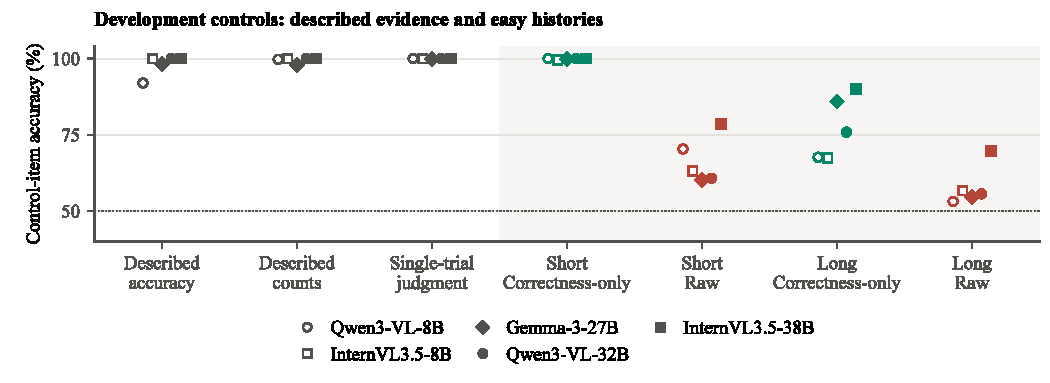
\includegraphics[width=\textwidth]{figures/fig_controls.pdf}
  \caption{Open models use directly stated evidence more reliably than easy raw histories. Development controls with text reports: described accuracy/counts, a single-trial correctness judgment, and easy short or long histories. Shading marks history-based items. Colour distinguishes raw and correctness-only histories; point shape and fill identify the five models. Accuracy here scores each control's requested answer, rather than the uncertain outcomes of the main task.}
  \label{fig:controls}
\end{figure*}

\paragraph{Control conditions.} Table~\ref{tab:controls_full} gives each control condition with text and image reports, and Table~\ref{tab:decomp} the stepwise differences between history formats on the main task. Image reports lowered accuracy in almost every control condition, including described accuracy (.59--.84 instead of .92--1.00); the one exception was Qwen3-VL-8B with a long raw history (.533 vs.\ .531). The image-report results use the selected icons (v3.1, Appendix~G), which every model named correctly on every single-image item (photos: .986--1.00), so these drops reflect the use of image reports rather than recognition of a single image. Control conditions were run on development episodes for all five models.

% FILL: analyze_controls.py on runs_h200/<model>/dev_controls -> pooled[control].hard_acc
\begin{table}[h]\centering\small
  \setlength{\tabcolsep}{2.2pt}
  \begin{tabular}{l ccccccc}
    \toprule
    & \multicolumn{2}{c}{Described} & \multicolumn{2}{c}{Short} & \multicolumn{2}{c}{Long} & Single \\
    \cmidrule(lr){2-3}\cmidrule(lr){4-5}\cmidrule(lr){6-7}
    Model & \% & counts & raw & corr. & raw & corr. & trial \\
    \midrule
    Qwen3-VL-8B & .920 & .998 & .703 & 1.00 & .531 & .676 & 1.00 \\
    InternVL3.5-8B & 1.00 & 1.00 & .632 & .996 & .567 & .674 & 1.00 \\
    Gemma-3-27B & .982 & .978 & .600 & 1.00 & .545 & .859 & 1.00 \\
    Qwen3-VL-32B & 1.00 & 1.00 & .607 & 1.00 & .556 & .759 & 1.00 \\
    InternVL3.5-38B & 1.00 & 1.00 & .786 & 1.00 & .696 & .900 & 1.00 \\
    \bottomrule
  \end{tabular}
  \caption{Control conditions on development episodes, text reports (accuracy on control items, averaged over counterbalanced copies; image reports in Appendix~C). Described: accuracy given as a percentage or as counts. Corr.: correctness only. Short/long: an easy history in which one advisor is clearly better, given raw or correctness-only. Single trial: who was correct on one shown trial. Full results by cover story in Appendix~C.}
  \label{tab:controls}
\end{table}

% FILL: analyze_controls.py -> table[] pooled over cover stories by report type (make_figures.load_controls); per cover story in the analysis output.
\begin{table*}[h]\centering\small
  \setlength{\tabcolsep}{4pt}
  \begin{tabular}{ll ccccc}
    \toprule
    Condition & Reports & Qwen3-8B & IVL-8B & Qwen3-32B & Gemma-27B & IVL-38B \\
    \midrule
    Described \% & Text & .920 & 1.00 & 1.00 & .982 & 1.00 \\
     & Image & .844 & .799 & .683 & .650 & .594 \\
    Described counts & Text & .998 & 1.00 & 1.00 & .978 & 1.00 \\
     & Image & .866 & .786 & .645 & .652 & .527 \\
    Short raw & Text & .703 & .632 & .607 & .600 & .786 \\
     & Image & .641 & .542 & .518 & .592 & .540 \\
    Short corr.\ only & Text & 1.00 & .996 & 1.00 & 1.00 & 1.00 \\
     & Image & .949 & .743 & .701 & .674 & .603 \\
    Long raw & Text & .531 & .567 & .556 & .545 & .696 \\
     & Image & .533 & .520 & .424 & .516 & .462 \\
    Long corr.\ only & Text & .676 & .674 & .759 & .859 & .900 \\
     & Image & .585 & .449 & .493 & .598 & .536 \\
    Single trial & Text & 1.00 & 1.00 & 1.00 & 1.00 & 1.00 \\
    \midrule
    Described \%, name on image & Image & .833 & .833 & .761 & .719 & .629 \\
    Described \%, composite image & Image & .750 & .853 & .766 & .810 & .969 \\
    Described \%, name after image & Image & .616 & .699 & .551 & .536 & .665 \\
    Composite read & Image & 1.00 & 1.00 & 1.00 & 1.00 & 1.00 \\
    Chart read & Chart & .620 & .688 & .672 & .609 & .708 \\
    \bottomrule
  \end{tabular}
  \caption{Control conditions on development episodes (accuracy on control items, averaged over counterbalanced copies and pooled over cover stories). Lower block: binding variants of the described-accuracy condition with image reports (advisor name printed on the image; both reports in one composite image; name given after the image), reading one panel of the composite image, and reading one cell of the correctness chart. Qwen3: Qwen3-VL; IVL: InternVL3.5. Image reports use the selected icons (v3.1). Results by cover story will be included in the released analysis output.}
  \label{tab:controls_full}
\end{table*}

% FILL: analyze_main.py held-out -> b_vs_a (A+, B, B' vs A: mean, ci95) and positions (C_minus_B, position, ci95, interpretable).
\begin{table*}[h]\centering\small
  \setlength{\tabcolsep}{3pt}
  \begin{tabular}{l cccccc c}
    \toprule
    Model & Raw+corr. & Corr.\ only & Chart acc. & Chart$-$raw & Summary$-$corr.\ only & Summary & Position \\
    \midrule
    Qwen3-VL-8B & +.031 & +.132 & .516 & +.030 & +.002 & +.134 & 0.98 [0.90, 1.07] \\
    InternVL3.5-8B & +.029 & +.157 & .534 & +.056 & $-$.001 & +.156 & 1.01 [0.96, 1.05] \\
    Gemma-3-27B & +.028 & +.132 & .559 & +.089 & +.016 & +.147 & 0.89 [0.83, 0.96] \\
    Qwen3-VL-32B & +.054 & +.160 & .583 & +.115 & +.003 & +.164 & 0.98 [0.93, 1.03] \\
    InternVL3.5-38B & +.011 & +.076 & .605 & +.056 & +.008 & +.084 & 0.90 [0.81, 1.01] \\
    \bottomrule
  \end{tabular}
  \caption{Chart accuracy and decomposition of the raw--summarized gap on held-out episodes. Chart acc. is absolute accuracy with the chart history; the other accuracy columns are paired differences from raw history, except Summary$-$correctness only. All accuracy quantities are proportions. Position: (correctness only $-$ raw)/(summary $-$ raw), with its 95\% bootstrap CI, reported only when the summary--raw gap exceeds the prespecified threshold and its CI excludes zero.}
  \label{tab:decomp}
\end{table*}
\subsection{D. Normative Simulation}                  % rule comparison across contrasts/phase lengths (design_sim)
We ran two simulations without any VLM to check the design. Both score a rule by the proportion of trials ($t \ge 2$) on which the advisor it favours is correct; ties score 0.5.

\paragraph{Design simulation.} The first simulation draws outcomes independently from the schedule (300 episodes per setting) and compares BOCPD (posterior predictive, $h \in \{1/8, 1/15, 1/30\}$), majority counts over the last $K \in \{3,5,7,10,15,20,30\}$ trials, counts over all past trials, and counts since the last true reversal. Across 20 settings (accuracy 0.65--0.85; phase lengths 40/40, 60/60 and 80/40; dwell 10 or 15 trials), the best BOCPD minus the best fixed window ranged from $-0.004$ to $+0.008$. For our setting (0.8; 40/40; dwell 10), accuracy was 0.687 for the best BOCPD ($h=1/8$), 0.683 for $h=1/15$, 0.690 for the best window ($K=3$), 0.632 for counts over all trials and 0.739 for counts since the last reversal. Conclusions were the same for accuracies from 0.65 to 0.85, and accuracy varied by about one percentage point for hazard rates between 1/8 and 1/30.

\paragraph{Rules given to the VLM.} The second simulation applies exactly the rules used to build the summarized histories (Appendix~E) to the actual episodes. Table~\ref{tab:normsim} gives the results. On held-out episodes, the 5-trial window (.692 [.685, .698]) is about 1.4 percentage points above the change-point summary (.678 [.666, .688]); counts over all trials (.632) are 6.0 points below the 5-trial window and 4.6 points below the change-point summary. On the robustness set, the 5-trial window (.675) again leads the change-point summary (.663) and the reversal-aligned reference is highest (.735), but the remaining rules are ordered differently: on held-out episodes counts over all trials (.632) exceed the 10-trial (.612) and 20-trial (.579) windows, whereas on the robustness set the 10-trial (.635) and 20-trial (.604) windows exceed counts over all trials (.594). These differences hold for the tested settings only; we do not claim that online rules are equivalent in general. The reversal-aligned summary uses only reversals up to $t-1$ and so learns of a reversal one trial late; it is a reference, not an upper bound on any strategy. Likewise, 0.8 is the accuracy of an observer who knows the current accuracy, not a strict ceiling (Appendix~B).

\begin{table}[h]
  \centering
  \small
  \setlength{\tabcolsep}{4pt}
  \begin{tabular}{lccc}
    \toprule
    Summary rule & Development & Held-out & Robustness \\
    \midrule
    All trials & .630 & .632 & .594 \\
    Last 5 trials & .698 & .692 & .675 \\
    Last 10 trials & .620 & .612 & .635 \\
    Last 20 trials & .578 & .579 & .604 \\
    Change-point (BOCPD) & .678 & .678 & .663 \\
    Since last reversal & .739 & .744 & .735 \\
    \bottomrule
  \end{tabular}
  \caption{Accuracy of the summary rules alone (no model) on development (16), held-out (48) and robustness (24) episodes. 95\% bootstrap CIs over episodes (2{,}000 resamples), held-out: last 5 trials [.685, .698]; change-point [.666, .688]; all trials [.628, .636].}
  \label{tab:normsim}
\end{table}

These rule baselines were computed on held-out episodes before any model results on the main data were seen. They are properties of the episode generator and involve no model behavior.

% FILL: analyze_main.py held-out -> baselines[].table (acc, ci95), on the same trial mask as the model runs.
\begin{table}[h]\centering\small
  \begin{tabular}{l cc}
    \toprule
    Baseline (no model) & Held-out & Robustness \\
    \midrule
    Always follow A & .648 & .547 \\
    Known current accuracy & .800 & .788 \\
    BOCPD posterior & .677 & .675 \\
    Outcome quota (knows block quota) & .655 & -- \\
    \bottomrule
  \end{tabular}
  \caption{Additional model-free baselines on the same trials as the models (95\% CIs in the analysis output). Always follow A and the outcome quota use generator information hidden from the models and are diagnostics, not strategies; the robustness set has no outcome quota.}
  \label{tab:baselines}
\end{table}
\subsection{E. Change-Point Controller and Summary Variants} % BOCPD details, hazard, K selection on dev
\paragraph{Change-point detection.} Let $o_t = 1$ if advisor A was correct on trial $t$. Before trial $t$, the controller runs Bayesian online change-point detection \citep{adams2007bocpd} on $o_1,\dots,o_{t-1}$ with a Bernoulli likelihood, a Beta(1,1) prior for each run and a constant hazard rate $h = 1/15$. This rate lies between the reversal rates of the volatile (1/10) and stable phases and was not tuned (Appendix~D). The controller takes the maximum a posteriori run length $r$ (the inferred number of trials since the last change), sets it to at least 3, and summarizes trials $\max(1, t-r)$ to $t-1$.

\paragraph{Summary variants.} All variants use the same sentence as the summarized history, restricted to a range of trials (``Summary of the last $n$ days (days $s$--$(t-1)$): Ken was correct $x$ times; Sam was correct $y$ times.''). The variants are: all past trials (the primary summary); the last $K \in \{5, 10, 20\}$ trials; the run since the last inferred change-point (BOCPD); and the trials since the last true reversal up to $t-1$ (reversal-aligned reference). Two further conditions truncate the raw history instead of summarizing it: to the BOCPD run, or to the last 10 trials. The window length used in the secondary tests is, for each model, the one with the highest accuracy on development episodes, fixed before held-out evaluation; Table~\ref{tab:variants} reports the selected length and all variants, and Table~\ref{tab:agree} compares the model with the rule alone. The last five trials were selected for every model. On held-out episodes, accuracy followed the rule in every variant: last 5 trials .667--.691 (rule alone .692), change point .666--.677 (.678), last 10 trials .605--.616 (.612), last 20 trials .581--.586 (.579). The model thus adds little to, and takes little from, the rule it is given; the choice of rule decides accuracy. The same holds for the reversal-aligned reference (.727--.744; rule alone .744). Truncating the raw history did not help: with only the last 10 raw trials, accuracy was .391--.467, at or below the full raw history (.468--.549) in every model, and truncating to the change-point run gave .472--.477 in the two 8B models. Shortening this raw format did not recover the benefit of stating who was correct.

% FILL: K* from dev_selection JSON (--write-dev-selection); accuracies from analyze_main.py held-out -> cells (C|sum_*|text, A|cp_hard|text, A|window:10|text).
\begin{table*}[h]\centering\small
  \setlength{\tabcolsep}{4pt}
  \begin{tabular}{l c cccccc cc}
    \toprule
    & & \multicolumn{6}{c}{Summarized history} & \multicolumn{2}{c}{Truncated raw history} \\
    \cmidrule(lr){3-8}\cmidrule(lr){9-10}
    Model & Selected $K$ & All trials & Last 5 & Last 10 & Last 20 & Change-point & Since reversal & Change-point & Last 10 \\
    \midrule
    Qwen3-VL-8B & 5 & .621 & .667 & .605 & .582 & .666 & .727 & .477 & .458 \\
    InternVL3.5-8B & 5 & .635 & .681 & .613 & .586 & .673 & .737 & .472 & .467 \\
    Gemma-3-27B & 5 & .617 & .677 & .609 & .581 & .667 & .728 & \tbd & .391 \\
    Qwen3-VL-32B & 5 & .631 & .691 & .615 & .582 & .675 & .740 & \tbd & .429 \\
    InternVL3.5-38B & 5 & .633 & .691 & .616 & .581 & .677 & .744 & \tbd & .450 \\
    \midrule
    Rule alone & -- & .632 & .692 & .612 & .579 & .678 & .744 & -- & -- \\
    \bottomrule
  \end{tabular}
  \caption{Main-task accuracy for every summary variant and the truncated raw histories (held-out). Rule alone: the summary's majority rule without a model (Table~\ref{tab:normsim}). Selected $K$: chosen on development episodes. Since reversal: uses the true reversal times, hidden from the models, and is a reference, not a strategy. Truncated raw histories have no rule (--). \todo{truncated change-point raw history for the three larger models}}
  \label{tab:variants}
\end{table*}

% FILL: analyze_main.py held-out -> tost[] (acc_vlm, acc_rule, mean, ci95) and agreement[] (agree_trial_pooled), domain=all.
\begin{table*}[h]\centering\small
  \setlength{\tabcolsep}{2pt}
  \begin{tabular}{ll cccc}
    \toprule
    Model & Summ. & VLM & Rule & $\Delta$ [90\% CI] & Agree \\
    \midrule
    Qwen3-VL-8B & All & .621 & .632 & $-$.011 [$-$.017, $-$.005] & .941 \\
     & CP & .666 & .678 & $-$.012 [$-$.017, $-$.007] & .970 \\
     & Selected & .667 & .692 & $-$.024 [$-$.034, $-$.015] & .943 \\
    InternVL3.5-8B & All & .635 & .632 & +.003 [.000, .006] & .978 \\
     & CP & .673 & .678 & $-$.005 [$-$.007, $-$.003] & .985 \\
     & Selected & .681 & .692 & $-$.011 [$-$.016, $-$.006] & .977 \\
    Gemma-3-27B & All & .617 & .632 & $-$.014 [$-$.019, $-$.010] & .935 \\
     & CP & .667 & .678 & $-$.011 [$-$.015, $-$.006] & .965 \\
     & Selected & .677 & .692 & $-$.015 [$-$.021, $-$.009] & .958 \\
    Qwen3-VL-32B & All & .631 & .632 & .000 [$-$.003, .002] & .994 \\
     & CP & .675 & .678 & $-$.003 [$-$.005, $-$.001] & .993 \\
     & Selected & .691 & .692 & $-$.001 [$-$.003, .000] & .997 \\
    InternVL3.5-38B & All & .633 & .632 & +.001 [$-$.001, .003] & .999 \\
     & CP & .677 & .678 & $-$.001 [$-$.001, .000] & 1.00 \\
     & Selected & .691 & .692 & .000 [$-$.001, .000] & 1.00 \\
    \bottomrule
  \end{tabular}
  \caption{VLM with summarized history vs.\ the summary's rule alone on identical held-out trials (CP: change point; Selected: last five trials). Agree: proportion of non-tied trials on which the model's choice equals the rule's. Equal accuracy does not imply the same strategy; agreement is reported for that reason.}
  \label{tab:agree}
\end{table*}

\paragraph{What the controller is.} The controller is a training-free rule outside the model; it sees only the sequence indicating whether advisor A was correct and does not read model states. It is motivated by change-point models of human learning \citep{nassar2010approximately,nassar2012rational}, but we use it as an integration rule, not as a model of the VLM or of the brain.
\begin{figure*}[t]\centering
  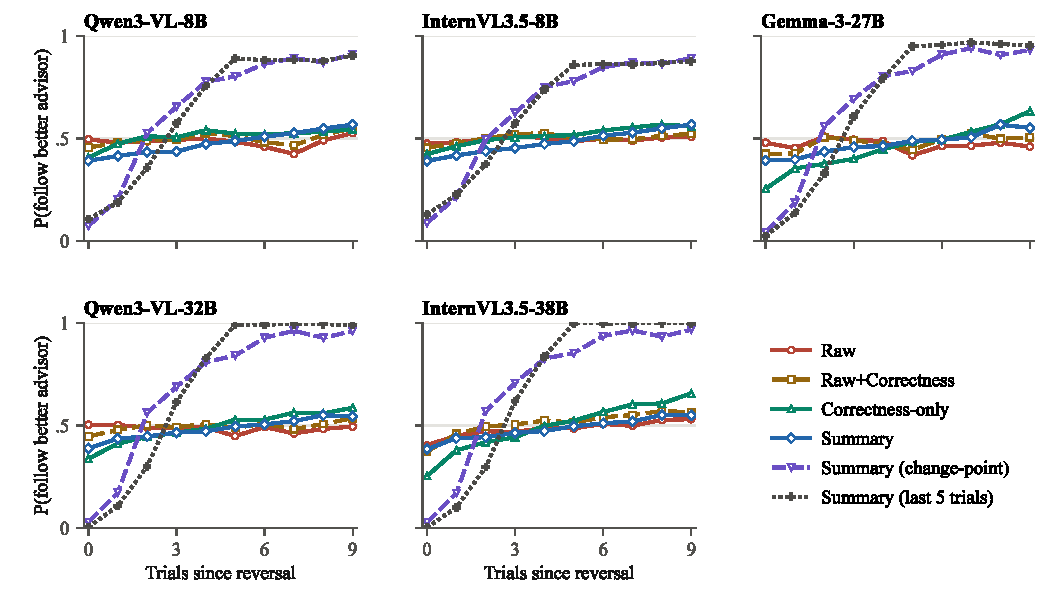
\includegraphics[width=\textwidth]{figures/fig_curves_models.pdf}
  \caption{Following the currently better advisor after a reversal, separately for each open model and history format. Each curve is a mean choice probability on held-out episodes; the panels are descriptive and do not show confidence intervals. Fig.~\ref{fig:curves} summarizes the same curves over the five fixed models.}
  \label{fig:curves_models}
\end{figure*}

\subsection{F. Computational Models and Parameter Recovery}  % delta-rule variants, calibrated learning rates, LOEO-CV
\paragraph{Models.} Let $o_t=1$ if advisor A was correct on trial $t$ and $y_t$ the model's choice probability for A. Each computational model maps $o_1,\dots,o_{t-1}$ to a belief $q_t$ that A is correct and predicts choice probability $P_t=\sigma(\beta(q_t-0.5)+b)$, where $\sigma$ is the logistic function, $\beta$ the inverse temperature and $b$ a bias. M0 is a constant bias ($P_t=\sigma(b)$). Win-stay/lose-shift follows the advisor who was correct on the previous trial ($P_t=\sigma(b+w(2o_{t-1}-1))$, with weight $w$). Count models use $q_t=(s+1)/(n+2)$, where $s$ counts A's correct reports among $n$ observed trials, using all past trials or the last $k$ trials. M1 is a delta rule, $q_{t+1}=q_t+\alpha(o_t-q_t)$ with learning rate $\alpha$ and $q_1=0.5$; M2 uses separate learning rates in the stable and volatile phases; M3 uses separate rates for outcomes that confirm or disconfirm the currently trusted advisor. M4 comprises a Bayesian change-point observer (hazard rate from a grid, or marginalized over it) and a volatility-tracking learner after \citet{behrens2007learning}, each either with a fitted readout or reading out its predictive probability directly.

\paragraph{Fitting and comparison.} Because $y_t$ is a choice probability rather than a sampled choice, models are fitted by minimizing the soft cross-entropy $-\sum_t [y_t\log P_t+(1-y_t)\log(1-P_t)]$, a pseudo-likelihood. Models are compared by leave-one-episode-out cross-validation: both cover-story versions of an episode are held out together, parameters are fitted on the other episodes, and losses are pooled across the two held-out versions. Uncertainty in the effective-learning-rate summary is computed across episode pairs after averaging the cover-story versions. Information criteria are reported only as heuristics. Following the analysis plan, learning-rate analyses are run only for conditions in which a model can use reliability at all (described accuracy $\ge 0.8$ in the control conditions) and tracks the better advisor in the stable phase (probability $\ge 0.6$); on development episodes, stable-phase following under raw histories was .53--.57 in every model, below this criterion, whereas it was .86--.98 with correctness-only and summarized histories.

\paragraph{Effective learning rate.} The update of the model's choice probability in logit space after each outcome, regressed on the signed outcome separately for the stable and volatile phases, measures how strongly the model responds to new outcomes. This statistic is not zero for a learner with a single constant learning rate: preferences are more extreme in the stable phase, where the logit stretches updates. We therefore calibrate it against a null in which M1, fitted to the same episode, generates simulated choice probabilities with the same residual noise (200 simulations); the calibrated volatile-minus-stable difference and its $z$ score against the null indicate whether a model updates more in the volatile phase than a constant-rate learner would.

\paragraph{Recovery.} In simulations with M1--M3 (100 synthetic learners each, logit noise s.d.\ 0.3), learning rates were recovered with correlations of .998 (M1; M2 stable and volatile rates) and .89--.99 (M3). Model identification was asymmetric: data from M1 were always classified as M1, but data from M2 were classified as M2 in 40\% of cases (70\% when the two rates differed by more than 0.2) and data from M3 rarely as M3 (10\%). The sign of the M2 rate difference was recovered in every case with a clear difference. Phase-specific rates are thus estimable, whereas model comparison favors the simpler M1 unless the difference is large; the calibrated effective learning rate is a separate diagnostic, whose ability to detect volatility adaptation on this schedule must also be checked (below). Table~\ref{tab:recovery} checks the strategy and kernel analyses of the main text on synthetic agents run on the same episodes.

% Prior development CV held out cover stories separately. Do not restore its loss/model-selection results before rerunning with episode-grouped folds.

\paragraph{Can these episodes reveal volatility-dependent learning?} We checked this with the Bayesian volatility learner of \citet{behrens2007learning}, which does learn faster when accuracy is volatile. On our 80-trial episodes its implied learning rate rose only from .100 in the stable to .115 in the volatile phase (held-out episodes). Neither the calibrated volatile-minus-stable effective learning rate ($+0.002$ [$-0.010$, $0.014$] over 16 development episodes) nor phase-specific integration kernels (volatile/stable ratio of the summed weight of the last three outcomes: 0.84--0.90, versus 0.96 for a constant-rate learner) detected this change, so we do not use the advice task to test whether models adapt their learning rate to volatility. The changing bandit (Appendix~I), in which volatility differs across whole games, tests that question instead.

% FILL: analyze_mechanism.py -> heuristics[<group>|<arm>]['all'][<heuristic>].kappa (+ kappa_ci95).
\begin{table*}[h]\centering\small
  \setlength{\tabcolsep}{4pt}
  \begin{tabular}{ll cccccc}
    \toprule
    Model & History & Repeat last outcome & Win-stay/lose-shift & Last 5 & All-trial counts & BOCPD & Label bias \\
    \midrule
    Qwen3-VL-8B & Raw & 0.22 & $-$0.01 & $-$0.01 & 0.01 & 0.00 & $-$0.14 \\
     & Summary & 0.00 & 0.06 & 0.15 & 0.24 & 0.16 & 0.01 \\
    InternVL3.5-8B & Raw & 0.26 & 0.05 & 0.02 & 0.01 & 0.03 & $-$0.02 \\
     & Summary & 0.01 & 0.06 & 0.15 & 0.45 & 0.15 & 0.00 \\
    Gemma-3-27B & Raw & 0.32 & 0.01 & $-$0.03 & 0.02 & $-$0.01 & 0.03 \\
     & Summary & 0.01 & 0.05 & 0.12 & 0.21 & 0.13 & 0.00 \\
    Qwen3-VL-32B & Raw & 0.24 & 0.00 & $-$0.03 & 0.01 & $-$0.02 & $-$0.17 \\
     & Summary & 0.01 & 0.05 & 0.12 & 0.80 & 0.13 & 0.01 \\
    InternVL3.5-38B & Raw & 0.13 & 0.07 & 0.11 & 0.04 & 0.12 & $-$0.03 \\
     & Summary & 0.01 & 0.06 & 0.12 & 0.98 & 0.13 & 0.01 \\
    \bottomrule
  \end{tabular}
  \caption{Agreement (Cohen's $\kappa$) between the model's choices and simple strategies (held-out). $\kappa$ corrects for chance agreement, so a rule that almost always picks one advisor can have high raw agreement and low $\kappa$. Repeat last outcome: predict the previous trial's outcome label. Win-stay/lose-shift: follow the advisor who was correct on the previous trial. Label bias: always predict the same label.}
  \label{tab:kappa}
\end{table*}

\begin{figure*}[h]\centering
  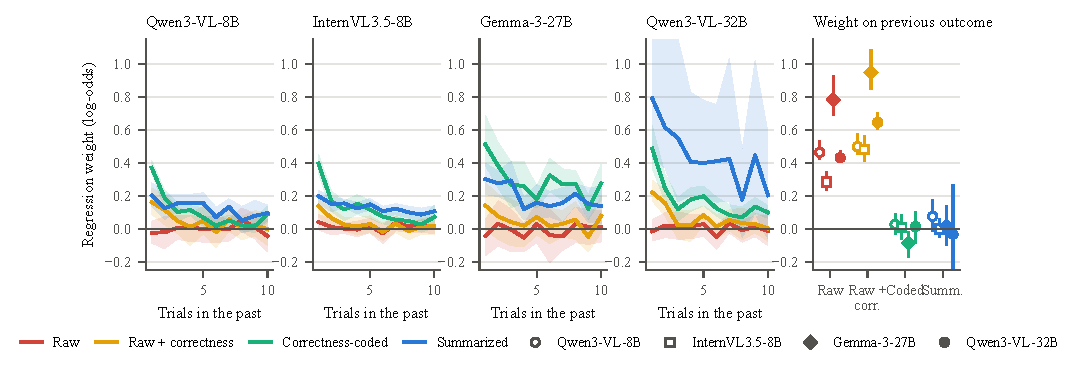
\includegraphics[width=\textwidth]{figures/fig_kernel_models.pdf}
  \caption{Integration kernels per model (shaded: 95\% bootstrap CI over episodes) and, bottom-right, the weight on repeating the previous outcome by history format (bars: 95\% CIs; held-out).}\label{fig:kernel_models}
\end{figure*}

% FILL: cogmodels.py LOEO-CV fits per model x history (NLL per trial, best model, effective learning rate in each phase).
\begin{table}[h]\centering\small
  \setlength{\tabcolsep}{3pt}
  \begin{tabular}{ll cccc}
    \toprule
    Model & History & Best & Loss/trial & Vol.$-$stable & $t$ \\
    \midrule
    Qwen3-VL-8B & Raw & \tbd & \tbd & \tbd & \tbd \\
     & Summary & \tbd & \tbd & \tbd & \tbd \\
    InternVL3.5-8B & Raw & \tbd & \tbd & \tbd & \tbd \\
     & Summary & \tbd & \tbd & \tbd & \tbd \\
    Gemma-3-27B & Raw & \tbd & \tbd & \tbd & \tbd \\
     & Summary & \tbd & \tbd & \tbd & \tbd \\
    Qwen3-VL-32B & Raw & \tbd & \tbd & \tbd & \tbd \\
     & Summary & \tbd & \tbd & \tbd & \tbd \\
    InternVL3.5-38B & Raw & \tbd & \tbd & \tbd & \tbd \\
     & Summary & \tbd & \tbd & \tbd & \tbd \\
    \bottomrule
  \end{tabular}
  \caption{Computational-model fits on held-out episodes: best model by leave-one-episode-out cross-validated soft cross-entropy per trial, and the calibrated volatile-minus-stable difference in effective learning rate with its across-episode $t$ statistic against zero. The latter is a descriptive diagnostic; the schedule does not reliably identify volatility adaptation.}
  \label{tab:cogfit}
\end{table}

% FILL: analyze_mechanism.py --validate -> validation[<dataset>][<agent>] (true params, recovered kernel / exp_fit).
\begin{table*}[h]\centering\small
  \setlength{\tabcolsep}{3pt}
  \begin{tabular}{l lc cc}
    \toprule
    Synthetic agent & Best strategy & $\kappa$ & Repeat $w$ & Lag-1 $w$ \\
    \midrule
    Repeat last outcome ($w=3$) & Repeat last outcome & 1.00 & 3.00 & 0.00 \\
    Delta rule ($\alpha=0.3$, $\beta=8$) & BOCPD & 0.94 & 0.00 & 1.20 \\
    50\% copy, 50\% delta & Repeat last outcome & 0.49 & 1.21 & 0.56 \\
    Last-5 counts & Last 5 & 1.00 & 0.02 & 1.08 \\
    All-trial counts & All-trial counts & 1.00 & 0.05 & 0.27 \\
    Label bias ($w=3$) & Label bias & 1.00 & 0.00 & 0.00 \\
    \bottomrule
  \end{tabular}
  \caption{Strategy and kernel analyses applied to synthetic agents on the main episodes (development and held-out; no VLM). Best strategy: highest Cohen's $\kappa$; Repeat $w$ and Lag-1 $w$: kernel regression weights on repeating the previous outcome and on the advisor correct one trial back. For the delta rule the fitted kernel decays geometrically with ratio 0.700 (true $1-\alpha=0.7$); the last-5 agent has a flat kernel up to lag 5. Strategies are correlated on this schedule, so the delta rule agrees best with BOCPD; the kernel, not the best-matching strategy, identifies it. Results on the robustness set were the same.}
  \label{tab:recovery}
\end{table*}
\begin{figure*}[t]\centering
  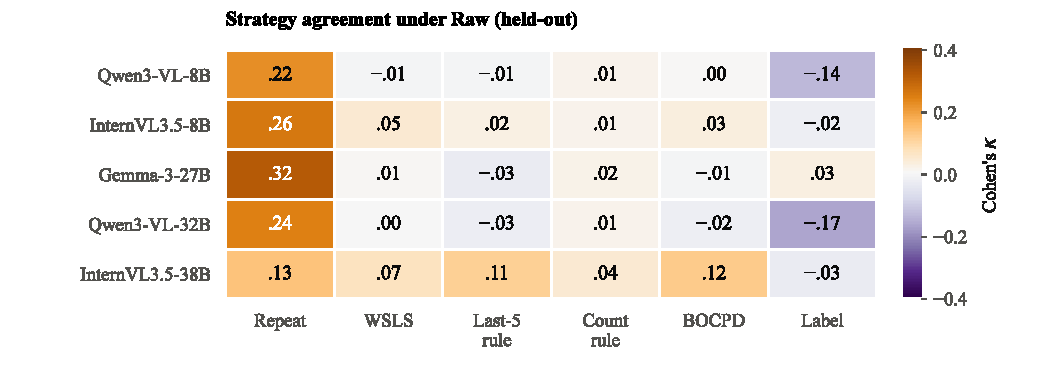
\includegraphics[width=\textwidth]{figures/fig_strategies.pdf}
  \caption{Under raw histories, repeating the previous outcome agrees most with the open models. Cohen's $\kappa$ on held-out episodes, with a colour scale centred at zero. Repeat: repeat the previous outcome; WSLS (win-stay/lose-shift): follow the advisor correct on the previous trial; Last 5 and Count: recent and all-trial correctness counts; BOCPD: change-point rule; Label: outcome-label bias. Values are rounded to two decimal places; rounding zeros has no effect on their colour.}
  \label{fig:strategies}
\end{figure*}

\subsection{G. Icon Design, Multimodal Binding and Chart Legibility}      % icon selection, image_named/composite/after, composite_read, chart_read
The legibility and binding controls use development episodes only and are exploratory; the comparison of text and image reports on the main task uses held-out episodes. All use the selected icons (v3.1) described below. Every model named every single report image correctly (InternVL3.5-8B: .986 for pet photos), so the remaining costs are not recognition failures (Table~\ref{tab:mm}). With described accuracy, accuracy in four models was lowest when the advisor's name was given only after the image (.54--.70) and higher when the name was printed on the image (.72--.83) or both reports were shown in one composite image (.75--.85), although each panel of a composite image was read correctly on every item; InternVL3.5-38B did best with the composite image (.97) and worst with plain image reports (.59). With correctness-only histories, image reports lowered held-out accuracy from .602--.636 to .523--.552. Reading a single cell of the correctness chart was below the prespecified 80\% chart-reading criterion for every model (.61--.71).

% FILL: analyze_controls.py (perception, composite_read, chart_read: hard_acc); analyze_main.py dev -> cells for report modality text / pet photo / icon and B' (chart).
\begin{table*}[h]\centering\small
  \setlength{\tabcolsep}{4pt}
  \begin{tabular}{l ccc ccc}
    \toprule
    & \multicolumn{3}{c}{Legibility controls} & \multicolumn{3}{c}{Main-task accuracy, correctness-only history} \\
    \cmidrule(lr){2-4}\cmidrule(lr){5-7}
    Model & Image naming & Composite read & Chart read & Text reports & Image reports & Chart history \\
    \midrule
    Qwen3-VL-8B & 1.000 & 1.000 & .620 & .619 & .552 & .516 \\
    InternVL3.5-8B & .988 & 1.000 & .688 & .636 & .544 & .534 \\
    Gemma-3-27B & 1.000 & 1.000 & .609 & .602 & .537 & .559 \\
    Qwen3-VL-32B & 1.000 & 1.000 & .672 & .628 & .527 & .583 \\
    InternVL3.5-38B & 1.000 & 1.000 & .708 & .625 & .523 & .605 \\
    \bottomrule
  \end{tabular}
  \caption{Multimodal reports (legibility controls on development episodes, exploratory; selected icons, v3.1). Image naming: single-image naming over all cover stories (photos and icons). Main-task columns: held-out episodes with correctness-only history, which removes outcome evaluation; because every model names the images, the drop with image reports reflects their use in context, including advisor binding. Chart history: correctness drawn as a chart (not interpreted, because chart read is below the prespecified 80\% chart-reading criterion for every model).}
  \label{tab:mm}
\end{table*}
\paragraph{Icon design and examples.} Icons replace the answer word with a picture in the image-report conditions. Figure~\ref{fig:icons} shows the actual deterministic renderings used in the icon probe, at 224 pixels; InternVL3.5 receives 448-pixel renderings from the same drawing functions. In the original medical pair, two red test-strip lines indicate positive and one indicates negative. The selected pair uses a dark plus or minus inside the same circular outline. In sports, the original gold trophy and red cross on a grey ball encode win and lose; the selected pair uses a yellow happy face and a grey-blue sad face. Labels and selection markers in the figure are reader annotations and are absent from the report images. These are synthetic symbols for the answer labels, not clinical scans or photographs of game outcomes. All other cover-story icons are unchanged.

\paragraph{Development-only selection.} We tested five medical pairs and four sports pairs with Qwen3-VL-8B and InternVL3.5-8B before held-out evaluation. The single-image probe asks for each of the two labels under both answer orders (four prompts per pair and model). We required all four responses to be correct for both models, then selected the eligible pair with the highest mean accuracy over four image-report controls and both models (Table~\ref{tab:icons}). The controls use described accuracy, a short raw history, a short correctness-only history, and a long correctness-only history. Each downstream cell contains 64 items after averaging label-aligned logits across the counterbalanced episode copies. This selected plus/minus and happy/sad faces. Enlarging the test strip left naming accuracy at .50 for both models, so size alone did not resolve that failure. Coloured plus/minus signs scored higher downstream but failed the InternVL3.5 naming criterion.

\paragraph{Results and limits.} The downstream mean increases from .521 to .668 for medical and from .588 to .678 for sports. Both selected pairs reach 4/4 in the naming probe for both models. However, accuracy in the described-accuracy condition, pooled over these two image-report cover stories is .773 for Qwen3-VL-8B and .727 for InternVL3.5-8B, below the 80\% described-accuracy criterion. Single-image recognition therefore does not establish successful use of image reports in the advice-taking task. Selection and evaluation use the same development controls, so these gains are descriptive and do not estimate held-out improvement.

\paragraph{Versioning and main-task check.} This development-driven change is a deviation from the fixed plan. The selected icons define v3.1; v3 remains reproducible and original outputs are retained separately. Text reports, pet photographs, the correctness chart, and the primary text-report comparison are unchanged. On the main task with correctness-only history and image reports (16 development episodes, both counterbalanced copies, trials $t\ge 2$), the selected icons raised mean accuracy over the original ones for both models: Qwen3-VL-8B from .51 to .62 (medical) and from .56 to .67 (sports), and InternVL3.5-8B from .50 to .55 and from .52 to .55 (paired differences over 32 episode copies: $+.11$ [.06, .16], $+.11$ [.09, .14], $+.05$ [.03, .06], $+.03$ [.02, .05]; 95\% bootstrap CIs). Accuracy remained below the same condition with text reports (Qwen3-VL-8B .57 and .70; InternVL3.5-8B .79 and .77), so image reports still add a cost beyond outcome evaluation, now with icons that both models name correctly. The selected icons also generalized beyond the two models used to choose them: Qwen3-VL-32B, InternVL3.5-38B and Gemma-3-27B named them correctly on every item. Tables~\ref{tab:controls_full} and~\ref{tab:mm} report the rerun with the selected icons.
% Evidence: runs/iconprobe/main_{plus_minus_faces,v3_strip_v3_trophy_x}_{q,i}; mean y over t>=2, not averaged over counterbalanced copies.

\begin{figure*}[t]\centering
  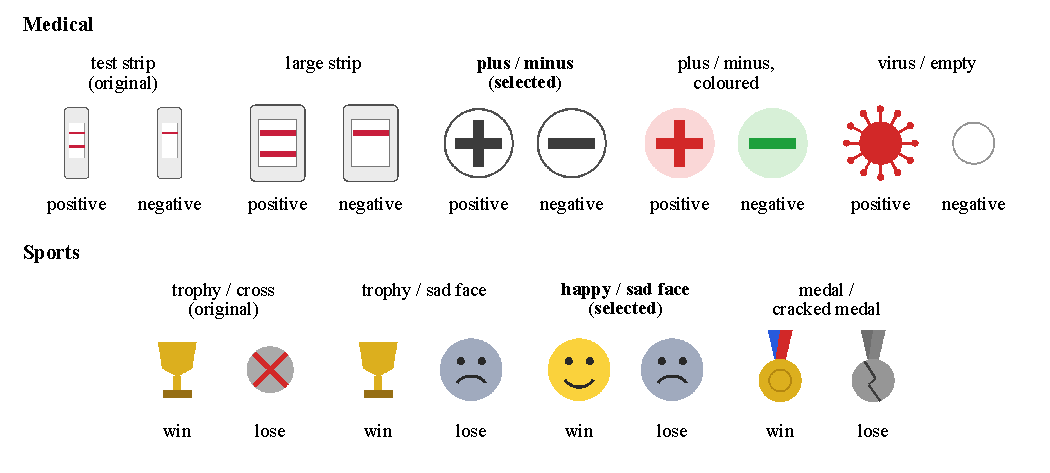
\includegraphics[width=\textwidth]{figures/fig_icons.pdf}
  \caption{Actual candidate report icons for medical (positive/negative) and sports (win/lose). Original marks the v3 pairs; selected marks their v3.1 replacements. Labels and headings are shown for the reader and are not embedded in model inputs. All candidates, including those not selected, are evaluated in Table~\ref{tab:icons}.}
  \label{fig:icons}
\end{figure*}

% Evidence: runs/iconprobe/{qwen3vl8b,internvl8b}.jsonl for the four-prompt probe;
% runs/iconprobe/ctl.json from analyze_controls.py for downstream controls averaged over counterbalanced copies.
\begin{table*}[t]\centering\small
  \setlength{\tabcolsep}{4pt}
  \begin{tabular}{l cccccc}
    \toprule
    Icon pair & Naming probe & Described \% & Short raw & Short corr.\ only & Long corr.\ only & Mean \\
    \midrule
    \multicolumn{7}{l}{\textit{Medical (positive / negative)}} \\
    Test strip (original) & .50/.50 & .61/.36 & .58/.62 & .62/.36 & .56/.45 & .52 \\
    Large test strip & .50/.50 & .61/.53 & .58/.59 & .73/.77 & .62/.56 & .62 \\
    Plus / minus (selected) & 1.00/1.00 & .70/.67 & .84/.62 & 1.00/.50 & .61/.39 & .67 \\
    Plus / minus, coloured & 1.00/.50 & .72/.70 & .77/.64 & 1.00/.95 & .61/.52 & .74 \\
    Virus / empty circle & .75/.75 & .61/.92 & .59/.59 & 1.00/.41 & .48/.39 & .62 \\
    \midrule
    \multicolumn{7}{l}{\textit{Sports (win / lose)}} \\
    Trophy / cross (original) & 1.00/.50 & .61/.64 & .52/.55 & .72/.62 & .61/.44 & .59 \\
    Trophy / sad face & 1.00/1.00 & .66/.73 & .55/.48 & .84/.83 & .61/.44 & .64 \\
    Happy / sad face (selected) & 1.00/1.00 & .84/.78 & .50/.52 & .80/1.00 & .50/.48 & .68 \\
    Medal / cracked medal & 1.00/.75 & .61/.64 & .53/.41 & .64/.39 & .48/.50 & .53 \\
    \bottomrule
  \end{tabular}
  \caption{Icon comparison on development items, image reports (Qwen3-VL-8B / InternVL3.5-8B). Naming probe: accuracy over two labels $\times$ two answer orders (four prompts per model and icon pair). Downstream columns: accuracy over 64 items per cell after averaging counterbalanced-copy logits; Described \% denotes described accuracy. Mean averages the four downstream conditions and both models, excluding the naming probe. Selection requires 4/4 naming accuracy for both models, then the highest mean.}
  \label{tab:icons}
\end{table*}

\subsection{H. Reasoning Mode}                               % thinking/CoT subset, lengths, truncation
Reasoning is tested on development episodes only, with each episode's own non-pet cover story and text reports. Qwen3-VL-8B-Thinking, the reasoning checkpoint of the same model family and size as Qwen3-VL-8B-Instruct, answers with its native reasoning template; the direct answers of Qwen3-VL-8B-Instruct on the same items are the reference. Because the two are different checkpoints, the comparison bounds what reasoning adds at this scale but does not isolate reasoning within one checkpoint; for compute reasons we did not run larger reasoning models or a step-by-step prompt. The subset comprises the main task at trials 20, 40, 60 and 80 with raw and summarized history, and the described-accuracy, short and long histories and their correctness-only versions at trials 40 and 80. Generation is greedy with up to 16{,}384 new tokens. We report free-answer accuracy, the valid-answer rate, truncation and forced-readout rates, and token cost separately; a probability read after the generated reasoning is conditional on that reasoning and is not compared directly with the direct-answer readout. Table~\ref{tab:reason} gives the results. \todo{one paragraph after results}

% FILL: analyze_thinking.py -> groups[<model/mode>][<condition>] (acc_valid, valid_rate, truncation_rate, forced_rate, tokens) and gap.
\begin{table*}[h]\centering\small
  \setlength{\tabcolsep}{4pt}
  \begin{tabular}{l cccc ccc c}
    \toprule
    & \multicolumn{4}{c}{Free-answer accuracy} & & & & \\
    \cmidrule(lr){2-5}
    Model / mode & Raw & Summary & Summary$-$raw & Described & Valid & Truncated & Forced & Median tokens \\
    \midrule
    Qwen3-VL-8B-Instruct, direct & \tbd & \tbd & \tbd & \tbd & -- & -- & -- & 1 \\
    Qwen3-VL-8B-Thinking & \tbd & \tbd & \tbd & \tbd & \tbd & \tbd & \tbd & \tbd \\
    \bottomrule
  \end{tabular}
  \caption{Reasoning subset (development episodes; main task at trials 20, 40, 60, 80; controls at 40 and 80). Direct: the instruction-tuned checkpoint's single-token answer on the same items. Accuracy is over valid generated answers. Valid: proportion of items with a valid generated answer. Truncated: proportion reaching the generation limit without finishing. Forced: proportion requiring an answer-token readout because no valid generated answer was available; these readouts are excluded from free-answer accuracy.}
  \label{tab:reason}
\end{table*}
\subsection{I. Psych-101 Protocol and Additional Fits}       % hidden/told, sampled-choice fits, long blocks, position
\paragraph{Task and data.} In the changing bandit of \citet{xiong2023neural}, participants repeatedly choose between two slot machines whose payoffs stay constant until a change point, which occurs with a hazard rate $h$; payoffs are noise-free, so a normative learner forgets the value of the unchosen machine at rate $\phi = h$. We use the 30 participants in Psych-101 \citep{binz2025foundation} and their three 100-trial games ($h = 0.1, 0.2, 0.4$; 90 games, 9{,}000 trials). Participants were told $h$, and each 100-trial game directly preceded a 1{,}500-trial game with the same $h$, so by their second and third 100-trial games participants had played 1{,}600 and 3{,}200 trials; models see each game on its own.

\paragraph{Replay.} Models are conditioned on each participant's previously executed behavior \citep{binz2025foundation}: before trial $t$ the model sees the original instructions and the participant's choices and payoffs on trials $1,\dots,t-1$, and is asked which machine to press (one letter). The readout is the choice probability between the two letters from the first-token logits, as in the main task. In the primary condition the hazard rate is removed from the instructions (hidden); in a secondary condition the original instructions state it (told). Model and participant thus share the within-game history but not the hazard information (hidden) or the prior experience (both conditions).

\paragraph{Fits.} We fit the myopic model-free learner of \citet{xiong2023neural}, which updates the chosen machine's value and forgets the unchosen one toward the midpoint at rate $\phi$, with a perseveration term capturing the effect of the previous choice, separately for each hazard rate. Humans give binary choices, so for comparability we draw 20 binary choice sequences from the model's choice probabilities in each game, fit each, and take the median. The primary statistic is each participant's slope of $\phi$ on $h$; the comparison is the paired difference between the model's and the human's slope (Wilcoxon test, participant-bootstrap 95\% CI), reported next to the model told versus human comparison and the model's told minus hidden contrast. The human fits are our re-analysis; \citet{xiong2023neural} report no learning rates by hazard rate. In our re-analysis, the median human $\phi$ rose from .079 ($h=0.1$) to .110 and .255 ($h=0.4$; per-participant slope 0.47 per unit $h$, positive in 73\% of participants, Wilcoxon $p=.008$), adjusting for game position did not remove the increase (0.64 [0.23, 1.05]), and in the following 1{,}500-trial games the increase was weaker (median $\phi$ .076, .114, .131; slope test $p=.029$).

\paragraph{Calibration of the human--model comparison.} We simulated the complete pipeline 200 times per condition. Simulated participants follow each real participant's fitted strategy at each hazard rate and play on the real value sequences; the simulated model follows the same strategy with its forgetting-rate slope shifted by $\delta$ and is replayed on the simulated participant's history; both are then fitted exactly as the real data (20 sampled choice sequences per model episode, median fit, paired Wilcoxon test and bootstrap CI). With $\delta = 0$, the test rejected at $p < .05$ in 6.0\% of replications (Monte Carlo standard error 1.7\%) and the 95\% CI covered the true difference in 93.5\%, but the estimated difference was biased upward by about $+0.09$. Power was 0.49 for $\delta = -0.5$ and 0.59 for $\delta = +0.5$, where CI coverage was 0.87 and 0.96. We therefore treat the comparison as supporting and descriptive (main text).

% FILL: psych101/analyze_xiong.py -> per_participant[M].phi by hazard, tests, paired slope difference (model - human), for hidden and told runs.
\begin{table*}[h]\centering\small
  \setlength{\tabcolsep}{4pt}
  \begin{tabular}{ll ccc c cc}
    \toprule
    & & \multicolumn{3}{c}{Median forgetting rate $\phi$} & & \multicolumn{2}{c}{Slope difference (model $-$ human)} \\
    \cmidrule(lr){3-5}\cmidrule(lr){7-8}
    Agent & Hazard info & $h=0.1$ & $h=0.2$ & $h=0.4$ & Slope & Est.\ [95\% CI] & $p$ \\
    \midrule
    Humans ($n=30$) & told & .079 & .110 & .255 & 0.47 & -- & -- \\
    \midrule
    Qwen3-VL-8B & hidden & .000 & .005 & .000 & $-$0.01 & $-$0.60 [$-$1.22, $-$0.05] & .021 \\
     & told & .000 & .018 & .000 & $-$0.01 & $-$0.59 [$-$1.00, $-$0.16] & .016 \\
    InternVL3.5-8B & hidden & .013 & .001 & .051 & 0.04 & $-$0.55 [$-$0.83, $-$0.14] & .070 \\
     & told & .024 & .010 & .029 & $-$0.04 & $-$0.61 [$-$0.92, $-$0.16] & .019 \\
    Gemma-3-27B & hidden & .000 & .000 & .000 & 0.00 & $-$0.55 [$-$1.38, $-$0.12] & .011 \\
     & told & .000 & .000 & .000 & 0.00 & $-$0.45 [$-$1.04, $-$0.06] & .014 \\
    Qwen3-VL-32B & hidden & .000 & .000 & .000 & 0.00 & $-$0.56 [$-$1.44, $-$0.13] & .031 \\
     & told & .000 & .000 & .000 & 0.00 & $-$0.57 [$-$1.57, $-$0.15] & .023 \\
    InternVL3.5-38B & hidden & .003 & .007 & .032 & 0.03 & $-$0.48 [$-$0.86, 0.04] & .025 \\
     & told & .004 & .002 & .062 & 0.16 & $-$0.44 [$-$0.84, 0.16] & .031 \\
    \bottomrule
  \end{tabular}
  \caption{Psych-101 changing bandit \citep{xiong2023neural}. Models are conditioned on each participant's history; $\phi$ is fitted to choices sampled from the model (20 draws, median). Slope: median over participants of the per-participant slope of $\phi$ on hazard rate (humans: our re-analysis). The paired test has power of about 0.5 and an upward bias of about $+0.09$ (calibration above), so it is descriptive only. The $p$-values shown are unadjusted; none of the five hidden-hazard comparisons survives Holm correction.}
  \label{tab:psych}
\end{table*}
\paragraph{Image and chart formats.} With the hazard rate hidden, the changing bandit is also run with the last five payoffs shown as pictures of the machine's display instead of text (224 px), and with the whole history drawn as one scatter chart of payoff by trial for each machine (448 px). Each has a perception check: reading the number on one machine picture (four options; 450 items), and reading which machine was pressed, or which gave more points, at a given trial of the chart (540 items). We report each format's fits next to its perception check, since a model that cannot read the pictures or the chart cannot be expected to learn from them. Every model read the number on a machine picture (.996--1.00), but none read the chart reliably (which machine was pressed: .56--.61; which gave more points: .50--.72), so chart results are not interpreted. With picture payoffs, forgetting rates stayed low (median at most .10) and did not rise with the hazard rate in four models (slopes $-0.20$ to $-0.00$); Gemma-3-27B was the exception (.000, .000, .087; slope 0.25, $p=.010$), still below the participants (paired difference $-0.23$ [$-1.02$, 0.21]).

\paragraph{Model-free check of forgetting (exploratory).} For every trial on which both machines had been observed, we regressed the choice of the first machine (participants: binary; models: choice probability) on the difference between the two machines' last observed values (per 10 points), separately when the older of the two values had been observed at most two trials earlier (fresh) or at least four trials earlier (stale), with the previous choice as a covariate (Table~\ref{tab:stale}). All models were sensitive to value. We resampled the 30 participants as whole clusters (2{,}000 replicates), refitting the regression and using the same sampled participants for each human--model comparison. The stale-minus-fresh coefficient was negative for participants at $h=0.1$ ($-.263$ [$-.501$, $-.114$]); its CIs included zero at the other hazards. Model-minus-human contrasts were positive at $h=0.1$ and $h=0.4$ in all five models (pointwise CIs above zero; Table~\ref{tab:stale}). This supports a difference in stale-value use under replay, without establishing a hazard-dependent adaptation deficit.

% Evidence: research/volatile_trust/analysis/h200_ho/reviewer_checks/summary.txt (analyze_reviewer_checks.py)
\begin{table*}[h]\centering\small
  \setlength{\tabcolsep}{5pt}
  \begin{tabular}{l ccc}
    \toprule
    & \multicolumn{3}{c}{Stale $-$ fresh value weight [95\% CI]} \\
    Agent (hazard hidden) & $h=0.1$ & $h=0.2$ & $h=0.4$ \\
    \midrule
    Participants (told) & $-$.263 [$-$.501, $-$.114] & $-$.049 [$-$.170, .046] & $-$.040 [$-$.122, .034] \\
    Qwen3-VL-8B & +.047 [$-$.037, .146] & $-$.009 [$-$.081, .080] & +.089 [.048, .133] \\
    InternVL3.5-8B & +.100 [.052, .147] & +.057 [.016, .101] & +.087 [.054, .119] \\
    Gemma-3-27B & +.049 [$-$.011, .110] & +.035 [$-$.016, .094] & +.053 [.007, .097] \\
    Qwen3-VL-32B & +.040 [$-$.017, .102] & +.026 [$-$.047, .097] & +.099 [.052, .138] \\
    InternVL3.5-38B & +.146 [.066, .229] & +.039 [$-$.020, .106] & +.105 [.070, .141] \\
    \midrule
    & \multicolumn{3}{c}{Model $-$ human contrast in stale $-$ fresh weight [95\% CI]} \\
    \midrule
    Qwen3-VL-8B & +.310 [.159, .552] & +.039 [$-$.063, .169] & +.129 [.049, .212] \\
    InternVL3.5-8B & +.363 [.216, .598] & +.105 [.021, .217] & +.127 [.055, .208] \\
    Gemma-3-27B & +.313 [.156, .541] & +.084 [$-$.007, .198] & +.093 [.014, .180] \\
    Qwen3-VL-32B & +.303 [.139, .557] & +.075 [$-$.024, .189] & +.140 [.071, .214] \\
    InternVL3.5-38B & +.410 [.236, .663] & +.087 [$-$.033, .225] & +.145 [.075, .226] \\
    \bottomrule
  \end{tabular}
  \caption{Exploratory stale-value regression. Coefficients are log-odds per 10 points of last-observed value difference. Negative stale-minus-fresh values indicate discounting of stale values. Pointwise 95\% CIs use 2{,}000 participant-cluster bootstrap refits; the same participants are resampled for paired model--human contrasts. These are descriptive, unadjusted intervals, separate from the primary hazard-slope tests.}
  \label{tab:stale}
\end{table*}

\subsection{J. Robustness, Prompt Wording and Masking}                                   % IID/irregular episodes; per-cover-story results
\paragraph{Robustness set and cover stories.} On the robustness set, where correctness and outcome labels are drawn independently on each trial and reversals are irregular, raw-history accuracy was .507--.520 in four models (near chance) and .559 in InternVL3.5-38B, and summaries reached .582--.595, close to the count rule on these episodes (.594). The summary$-$raw gap was smaller than on the main set but positive and significant in every model ($+.036$ to $+.083$, Holm-corrected $p<.001$; Table~\ref{tab:robust}), so it does not depend on the outcome quotas. On held-out episodes the gap was positive in every non-pet cover story for every model (sign test $p=.031$, the smallest attainable) and in the pet cover story ($+.080$ to $+.179$; Table~\ref{tab:scenario}); it was smallest for Gemma-3-27B with the medical and news cover stories ($+.036$, $+.047$).

% FILL: analyze_main.py on robust_v3 runs -> gaps (C|sum_all vs A, domain=all): A/C acc, mean, ci95, p_wilcoxon.
\begin{table}[h]\centering\small
  \setlength{\tabcolsep}{3pt}
  \begin{tabular}{l ccc c}
    \toprule
    Model & Raw & Summary & Gap [95\% CI] & $p$ \\
    \midrule
    Qwen3-VL-8B & .507 & .582 & +.075 [.052, .100] & $<$.001 \\
    InternVL3.5-8B & .520 & .594 & +.074 [.042, .105] & $<$.001 \\
    Gemma-3-27B & .507 & .590 & +.083 [.055, .113] & $<$.001 \\
    Qwen3-VL-32B & .516 & .593 & +.077 [.051, .102] & $<$.001 \\
    InternVL3.5-38B & .559 & .595 & +.036 [.021, .051] & $<$.001 \\
    \bottomrule
  \end{tabular}
  \caption{Primary comparison on the robustness set (24 episodes with independent outcomes and irregular reversals); $p$: Wilcoxon signed-rank test, all Holm-corrected $p<.001$ within this family.}
  \label{tab:robust}
\end{table}

% FILL: analyze_main.py held-out -> scenarios[] (per_scenario mean, sign_test); pet from domain=pet gaps.
\begin{table*}[h]\centering\small
  \setlength{\tabcolsep}{4pt}
  \begin{tabular}{l cccccc c c}
    \toprule
    & \multicolumn{6}{c}{Non-pet cover stories} & & \\
    \cmidrule(lr){2-7}
    Model & Color & Weather & Stock & Sports & Medical & News & Sign test $p$ & Pet \\
    \midrule
    Qwen3-VL-8B & +.109 & +.095 & +.157 & +.131 & +.097 & +.134 & .031 & +.148 \\
    InternVL3.5-8B & +.172 & +.157 & +.136 & +.117 & +.101 & +.116 & .031 & +.179 \\
    Gemma-3-27B & +.160 & +.146 & +.171 & +.157 & +.036 & +.047 & .031 & +.175 \\
    Qwen3-VL-32B & +.169 & +.187 & +.193 & +.158 & +.168 & +.101 & .031 & +.164 \\
    InternVL3.5-38B & +.055 & +.101 & +.127 & +.087 & +.087 & +.068 & .031 & +.080 \\
    \bottomrule
  \end{tabular}
  \caption{Summary$-$raw gap by cover story (held-out; eight episodes per non-pet cover story). Pet: the pet cover story, shown in every episode alongside its other cover story (text reports here; photographs only in image-report conditions); it is not part of the sign test.}
  \label{tab:scenario}
\end{table*}

\begin{figure*}[t]\centering
  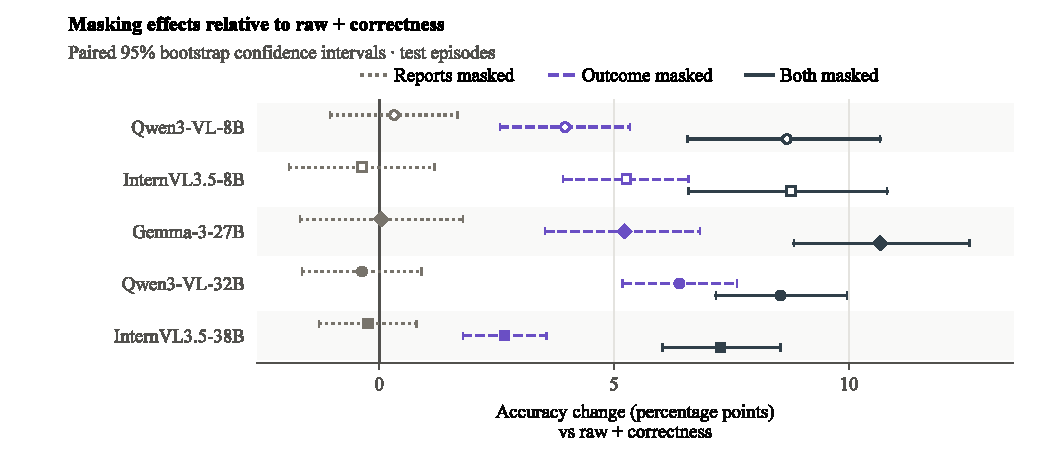
\includegraphics[width=\textwidth]{figures/fig_masking_effects.pdf}
  \caption{Paired masking effects corresponding to Fig.~\ref{fig:kernel}b. Each contrast compares masking the reports, the outcome, or both against the raw history with correctness appended; correctness statements remain visible. Points show accuracy changes in percentage points, with pointwise 95\% bootstrap CIs over the same 48 held-out episode pairs (10{,}000 resamples; text reports). The vertical line marks zero change. These are intervals for paired differences, not for the absolute accuracies in Fig.~\ref{fig:kernel}b.}
  \label{fig:masking_effects}
\end{figure*}

\paragraph{Which part of the raw history blocks the correctness statement.} Appending who was correct to the raw history recovered only part of the summary--raw gap, and the weight on repeating the previous outcome stayed large. To find out why, we kept the layout and length of that history and replaced parts of each past trial with a dash (``Day 3: Ken forecasts ---; Sam forecasts ---. Actual weather: rain. (Ken was correct; Sam was wrong.)''): the outcome label, the two reports, or both. With both replaced the history carries the same information as the correctness-only history at nearly the length of the raw history with correctness. On development episodes (Table~\ref{tab:mask}), replacing the outcome label raised accuracy by 7.4 and 9.6 points (main effects; 95\% CIs [5.2, 9.5] and [7.6, 11.5]) and lowered the weight on the previous outcome from .48--.50 to .12, whereas replacing the reports had no effect on its own ($+1.1$ and $-0.2$ points). With both replaced, accuracy was 1.5--2.1 points below the correctness-only history, leaving 14--20\% of the original accuracy difference despite retaining much of the surrounding text; this comparison does not isolate additive contributions of length, layout and outcome labels. The outcome label thus elicits repeating the previous outcome even when who was correct is stated. Predictions for the held-out replication in five models were written before it was run. On held-out episodes (Table~\ref{tab:mask}) all four predictions held in all five models. Replacing the outcome label raised accuracy over the raw history with correctness ($+2.7$ to $+6.4$ points; all $p<.001$) and cut the weight on the previous outcome from .42--.87 to .08--.23, whereas replacing the reports showed no clear accuracy change (between $-0.4$ and $+0.3$ points; all 95\% CIs include zero) and left that weight at .26--.65. Averaged over the other factor, replacing the outcome label had a larger effect than replacing the reports in every model (difference of main effects $+2.9$ to $+6.8$ points, all CIs above zero). With both replaced, accuracy was $+7.3$ to $+10.7$ points above the raw history with correctness and within $-4.0$ to $+0.8$ points of the correctness-only history, despite retaining the longer layout. The held-out effect of replacing the outcome label alone is smaller than on development episodes and recovers 40--60\% of the difference between the raw history with correctness and the correctness-only history.

% Evidence: research/volatile_trust/analysis/masking/summary.txt (analyze_masking.py; runs/masking/*); held-out: analyze_masking.py --root runs_h200 --split ho.
\begin{table*}[h]\centering\small
  \setlength{\tabcolsep}{4pt}
  \begin{tabular}{l cc cc cc cc cc}
    \toprule
    & \multicolumn{2}{c}{Raw + correctness} & \multicolumn{2}{c}{Reports shown} & \multicolumn{2}{c}{Outcome shown} & \multicolumn{2}{c}{Both replaced} & \multicolumn{2}{c}{Correctness only} \\
    \cmidrule(lr){2-3}\cmidrule(lr){4-5}\cmidrule(lr){6-7}\cmidrule(lr){8-9}\cmidrule(lr){10-11}
    Model & Acc. & Repeat & Acc. & Repeat & Acc. & Repeat & Acc. & Repeat & Acc. & Repeat \\
    \midrule
    \multicolumn{11}{l}{\textit{Development episodes}} \\
    Qwen3-VL-8B & .534 & .50 & .576 & .12 & .513 & .48 & .620 & .04 & .640 & .03 \\
    InternVL3.5-8B & .530 & .48 & .602 & .12 & .504 & .27 & .625 & .02 & .640 & .01 \\
    \midrule
    \multicolumn{11}{l}{\textit{Held-out episodes}} \\
    Qwen3-VL-8B & .517 & .44 & .557 & .08 & .520 & .40 & .604 & .01 & .619 & .02 \\
    InternVL3.5-8B & .508 & .44 & .561 & .10 & .504 & .26 & .596 & .03 & .636 & .02 \\
    Gemma-3-27B & .498 & .87 & .550 & .18 & .499 & .65 & .605 & .04 & .602 & .00 \\
    Qwen3-VL-32B & .522 & .60 & .586 & .13 & .518 & .60 & .607 & .02 & .628 & .00 \\
    InternVL3.5-38B & .560 & .42 & .586 & .23 & .557 & .37 & .633 & .02 & .625 & .01 \\
    \bottomrule
  \end{tabular}
  \caption{Masking parts of the raw history with correctness (text reports; accuracy uses pair-averaged label-aligned logits, $t\ge 2$). Reports shown: outcome label replaced; Outcome shown: reports replaced; Both replaced: same information as the correctness-only history. Repeat: regression weight on repeating the previous outcome. Development rows are exploratory (RTX 3090); held-out predictions were fixed beforehand and all held in all five models: replacing the outcome label raises accuracy, replacing both beats the raw history with correctness, and replacing the outcome label matters more than replacing the reports.}
  \label{tab:mask}
\end{table*}

\paragraph{Prompt wording (exploratory, development episodes).} We re-ran the four text history formats for Qwen3-VL-8B and InternVL3.5-8B with two alternative wordings; episodes, names, answer words, list order and readout were unchanged. Reworded sentences keep the original layout with different phrasing (``In trial 3, Sam said cat and Ken said dog; it turned out cat.''; ``Tally over the 3 previous trials: Ken was right 2 times and Sam was right 1 times.''). A compact record uses one line per trial (``\#3 | Sam=cat | Ken=dog | truth=cat''; ``Correct counts so far (3 trials): Ken=2, Sam=1.''). Table~\ref{tab:wording} gives the results. With reworded sentences, every result was preserved: raw history at .47--.49, summary$-$raw $+.12$ and $+.15$, the correctness-only history at or above the summary, appending correctness recovering about 40\% of the gap, and a positive weight on the previous outcome. The compact record changed the picture in both directions. Raw-history accuracy rose to .55--.56 and the weight on the previous outcome fell, whereas the correctness-only and summarized formats fell to .56--.60, and InternVL3.5-8B followed the count summary on only 72\% of non-tied trials (98\% with the original wording). The summary$-$raw gap shrank to $+.03$ [.01, .06] (Qwen3-VL-8B) and $+.01$ [$-.02$, .05] (InternVL3.5-8B). Raw-history accuracy stayed below the count rule (.63) in every wording, but the size of the raw--summarized gap depends on how the history is laid out, and we interpret it only for the natural-language layout used in all main conditions. The compact record is also run for the three larger models. \todo{larger models, compact record}

\paragraph{Which part of the compact record matters.} The compact record changes three parts of the prompt: the task description, the history lines together with the count summary, and the current-trial line together with the question. We crossed the original and compact version of each part ($2^3$ prompts; the all-original prompt reproduces the runner's prompts byte for byte; Table~\ref{tab:wordfact}). No single part accounts for the change. Each compact part, on its own, lowered the summary$-$raw gap by 0.3--5.4 points (main effects of 2.7--6.3 points), and the gap stayed positive with a 95\% CI above zero in all six mixed prompts. The largest single changes were these: the compact question lowered accuracy with the correctness-only history (main effect $-3.6$ and $-4.3$ points); the compact task description and count notation lowered agreement with the count rule (InternVL3.5-8B: $-8.6$ and $-10.2$ points); and for InternVL3.5-8B raw-history accuracy rose mainly when both the history lines and the current trial used the same one-line record (.477 and .491 with either alone, .559 with both). This last pattern fits the outcome-evaluation account: the gain under the raw history appeared when each past trial's reports and outcome were aligned in the same layout as the current reports, which makes deciding who was correct easier.

% Evidence: analysis/paraphrase/summary.txt (main effects) and paraphrase.json; runs/paraphrase/H*-L*-Q*_*.
\begin{table*}[h]\centering\small
  \setlength{\tabcolsep}{3.5pt}
  \begin{tabular}{ccc cccc cccc}
    \toprule
    & & & \multicolumn{4}{c}{Qwen3-VL-8B} & \multicolumn{4}{c}{InternVL3.5-8B} \\
    \cmidrule(lr){4-7}\cmidrule(lr){8-11}
    Task & History & Question & Raw & Corr.\ only & Summ. & Summ.$-$raw [95\% CI] & Raw & Corr.\ only & Summ. & Summ.$-$raw [95\% CI] \\
    \midrule
    O & O & O & .485 & .640 & .617 & $+.132$ [.108, .153] & .471 & .640 & .628 & $+.157$ [.140, .174] \\
    O & O & T & .512 & .613 & .627 & $+.115$ [.093, .137] & .491 & .604 & .617 & $+.126$ [.106, .146] \\
    O & T & O & .494 & .633 & .623 & $+.129$ [.114, .145] & .477 & .637 & .600 & $+.122$ [.099, .145] \\
    O & T & T & .532 & .588 & .608 & $+.076$ [.051, .105] & .559 & .616 & .597 & $+.038$ [.007, .065] \\
    T & O & O & .506 & .637 & .600 & $+.094$ [.066, .121] & .507 & .634 & .610 & $+.103$ [.073, .132] \\
    T & O & T & .520 & .599 & .600 & $+.080$ [.052, .108] & .493 & .562 & .600 & $+.107$ [.079, .131] \\
    T & T & O & .526 & .616 & .600 & $+.074$ [.040, .104] & .515 & .634 & .583 & $+.068$ [.035, .100] \\
    T & T & T & .563 & .580 & .597 & $+.034$ [.008, .059] & .550 & .593 & .564 & $+.014$ [$-$.019, .045] \\
    \bottomrule
  \end{tabular}
  \caption{Decomposition of the compact record (development episodes, text reports; accuracy averaged over counterbalanced copies, $t \ge 2$). O: original wording of that part; T: compact version. Task: task description; History: history lines and count summary; Question: current-trial line and question. The first row is the original prompt and the last row the compact record of Table~\ref{tab:wording}.}
  \label{tab:wordfact}
\end{table*}

% Evidence: research/volatile_trust/analysis/paraphrase/summary.txt (analyze_paraphrase.py; runs/paraphrase/*).
\begin{table*}[h]\centering\small
  \setlength{\tabcolsep}{5pt}
  \begin{tabular}{ll cccc c c}
    \toprule
    Model & Wording & Raw & Raw+c. & Corr.\ only & Summ. & Summ.$-$raw [95\% CI] & Repeat \\
    \midrule
    Qwen3-VL-8B & Original & .485 & .534 & .640 & .617 & $+.132$ [.108, .153] & .46 \\
    & Reworded & .488 & .533 & .624 & .607 & $+.119$ [.093, .144] & .50 \\
    & Compact & .563 & .561 & .580 & .597 & $+.034$ [.008, .059] & .32 \\
    \midrule
    InternVL3.5-8B & Original & .471 & .530 & .640 & .628 & $+.157$ [.140, .174] & .28 \\
    & Reworded & .473 & .538 & .644 & .627 & $+.153$ [.133, .175] & .26 \\
    & Compact & .550 & .559 & .593 & .564 & $+.014$ [$-.019$, .045] & .13 \\
    \bottomrule
  \end{tabular}
  \caption{Prompt-wording check (development episodes, text reports; accuracy averaged over counterbalanced copies, $t\ge 2$). Repeat: regression weight on the previous outcome under the raw history.}
  \label{tab:wording}
\end{table*}
\paragraph{Judgment question and report position (exploratory).} On raw-history trials the models were also asked which advisor was currently more likely to be correct (Appendix~K). Table~\ref{tab:judgpos} compares the judgment averaged over counterbalanced copies with the choice on the same trials, and gives, for image and text reports with the correctness-only history, the share of choices for the first-listed report and accuracy by the position of the correct report. Within each trial the two reports are listed in random order, identical in both counterbalanced copies.

% Evidence: research/volatile_trust/analysis/h200_ho/reviewer_checks/summary.txt (analyze_reviewer_checks.py)
\begin{table*}[h]\centering\small
  \setlength{\tabcolsep}{3.5pt}
  \begin{tabular}{l ccc c cc cc}
    \toprule
    & \multicolumn{4}{c}{Raw history, text reports} & \multicolumn{4}{c}{Correctness-only history} \\
    \cmidrule(lr){2-5}\cmidrule(lr){6-9}
    & Judgment & Choice & Choice follows & & \multicolumn{2}{c}{Chose first listed} & \multicolumn{2}{c}{Image: acc.\ when correct is} \\
    \cmidrule(lr){6-7}\cmidrule(lr){8-9}
    Model & names better & follows better & own judgment & $\kappa$ & Text & Image & first & second \\
    \midrule
    Qwen3-VL-8B & .633 & .523 & .579 & .09 & .455 & .523 & .571 & .525 \\
    InternVL3.5-8B & .674 & .524 & .527 & $-$.02 & .526 & .803 & .847 & .243 \\
    Gemma-3-27B & .602 & .531 & .576 & .07 & .438 & .792 & .828 & .243 \\
    Qwen3-VL-32B & .607 & .532 & .537 & .00 & .537 & .918 & .941 & .105 \\
    InternVL3.5-38B & .672 & .633 & .691 & .12 & .524 & .903 & .920 & .114 \\
    \bottomrule
  \end{tabular}
  \caption{Judgment and report position (held-out; averaged over counterbalanced copies). Names/follows better: the scheduled better advisor; always naming the advisor that is better over most of the episode scores .75. $\kappa$: agreement between judgment and choice. With raw histories and image reports, the larger models chose the first-listed image on .88--.93 of trials (text .57--.58).}
  \label{tab:judgpos}
\end{table*}

\subsection{K. Models, Revisions and Compute}                % pinned revisions, hardware
\begin{table}[h]
  \centering
  \small
  \setlength{\tabcolsep}{4pt}
  \begin{tabular}{llrl}
    \toprule
    Model & Family & Params & Image input \\
    \midrule
    Qwen3-VL-8B & Qwen3 & 8B & 224 px \\
    InternVL3.5-8B & Qwen3 & 8B & 448 px \\
    Gemma-3-27B & Gemma 3 & 27B & 896 px$^{a}$ \\
    Qwen3-VL-32B & Qwen3 & 32B & 224 px \\
    InternVL3.5-38B & Qwen3 & 38B & 448 px \\
    \midrule
    Qwen3-VL-8B-Thinking$^{b}$ & Qwen3 & 8B & 224 px \\
    \bottomrule
  \end{tabular}
  \caption{Models (used without fine-tuning; pinned revisions in Table~\ref{tab:revisions}). Family denotes the underlying language model; B denotes billions of parameters. Top block: core models (instruction-tuned). InternVL3.5: one 448-px tile. $^{a}$224-px renders resized by the processor. $^{b}$Reasoning subset only.}
  \label{tab:models}
\end{table}

Table~\ref{tab:models} lists the models and Table~\ref{tab:revisions} the Hugging Face checkpoints and pinned revisions. A 72B model was planned as a scale extension and larger reasoning models as a supplement, but neither was run for compute reasons.

\begin{table*}[t]
  \centering
  \small
  \begin{tabular}{lll}
    \toprule
    Model & Checkpoint & Revision \\
    \midrule
    Qwen3-VL-8B & Qwen/Qwen3-VL-8B-Instruct & 0c351dd01ed87e9c1b53cbc748cba10e6187ff3b \\
    InternVL3.5-8B & OpenGVLab/InternVL3\_5-8B-HF & 741a7d03020411e666c6109218ab71e08151ef86 \\
    Gemma-3-27B & google/gemma-3-27b-it & 005ad3404e59d6023443cb575daa05336842228a \\
    Qwen3-VL-32B & Qwen/Qwen3-VL-32B-Instruct & 0cfaf48183f594c314753d30a4c4974bc75f3ccb \\
    InternVL3.5-38B & OpenGVLab/InternVL3\_5-38B-HF & 7c830fc25e874f9a861087e3c70587f2b9b555f3 \\
    Qwen3-VL-8B-Thinking & Qwen/Qwen3-VL-8B-Thinking & 92f3c4b4feadd3a016ef468d103bb5f58b2a2c6b \\
    \bottomrule
  \end{tabular}
  \caption{Checkpoints and pinned revisions (resolved 2026-11-11).}
  \label{tab:revisions}
\end{table*}

\paragraph{Proprietary models.} GPT-6-Astra and Claude Fable 5.2 are queried through their APIs with the same prompts as the open models (text reports only), on a subset of held-out episodes and query trials: episodes 0--23 of the held-out set with their counterbalanced copies (four per non-pet cover story, half starting with each phase), every fourth trial ($t=4,8,\dots,80$), and the raw, correctness-only and all-trial summarized histories, 2{,}880 calls per model. Both were queried on 2026-11-13 with the default sampling settings (Claude Fable 5.2 does not accept a temperature), reasoning effort `low' (the lowest that GPT-6-Astra accepts; Claude Fable 5.2 always reasons) and at most 4{,}000 output tokens; Claude Fable 5.2 was queried through the Message Batches API. The served model identifiers were gpt-6-astra and claude-fable-5-2 on every call. The choice is the answer word: either the whole answer has at most three words and contains exactly one of the two answer words, or its last line is one of them; all other answers are invalid. GPT-6-Astra answered with one word on every call (median 5 output tokens, including reasoning); Claude Fable 5.2 gave visible reasoning before a final-line answer on 47\% of calls (77\% with raw histories; median 47 output tokens), and 6 of its 2{,}880 answers (0.2\%) were invalid. Because the readout differs from the two-token choice probability of the open models and the subset is smaller, these results are reported separately.

\paragraph{Behaviour of the proprietary models (exploratory).} To ask whether the proprietary models' raw-history accuracy reflects tracking the advisors or a shortcut, we computed, on the same items and with per-copy choices for all models, agreement with simple strategies, the choice on trials where two strategies disagree, the proportion following the currently better advisor by trials since the last reversal, and a logistic regression of following advisor A on A's correctness at lags 1--10 and on the repeat-previous-outcome regressor (Table~\ref{tab:apibeh}). The outcome-quota rule uses the generator's hidden 5/5 outcome quota and is a diagnostic only. With raw histories both proprietary models gave large, decaying weights to past correctness (lag 1: 2.1 and 3.3 log-odds; lag 5: 0.7 and 1.4) and no reliable weight on the previous outcome; the open models' weights on past correctness were near zero and their weight on the previous outcome positive.

% Evidence: research/volatile_trust/analysis/api_behavior/summary.txt (analyze_api_behavior.py)
\begin{table*}[h]\centering\small
  \setlength{\tabcolsep}{3.5pt}
  \begin{tabular}{l l c ccccc c cc}
    \toprule
    & & & \multicolumn{5}{c}{Agreement with strategy ($\kappa$)} & Quota vs.\ learner & \multicolumn{2}{c}{Since reversal} \\
    \cmidrule(lr){4-8}\cmidrule(lr){10-11}
    Model & History & Acc. & Repeat & WSLS & Count & Last 5 & Learner & follows learner & 1--3 & 8--10 \\
    \midrule
    Claude Fable 5.2 & Raw & .629 & .02 & .43 & .12 & .79 & .87 & .96 & .06 & .94 \\
    & Summary & .585 & .02 & .05 & 1.00 & .11 & .13 & .82 & .50 & .49 \\
    GPT-6-Astra & Raw & .628 & $-$.03 & .41 & .09 & .77 & .78 & .91 & .09 & .99 \\
    & Summary & .585 & .02 & .05 & 1.00 & .11 & .13 & .82 & .50 & .49 \\
    \midrule
    Open models (5) & Raw & .467--.503 & .08--.31 & .00--.04 & .01--.05 & $-$.01--.06 & .01--.08 & .59--.80 & .47--.56 & .43--.51 \\
    & Summary & .533--.590 & .01--.02 & .01--.07 & .04--.68 & .09--.16 & .08--.17 & .67--.81 & .47--.51 & .51--.58 \\
    \midrule
    Rule alone & & \multicolumn{9}{l}{repeat .458; WSLS .623; count .585; last 5 .679; learner .629; outcome quota (hidden) .702} \\
    \bottomrule
  \end{tabular}
  \caption{Behaviour on the API subset (24 episode pairs, $t=4,8,\dots,80$; per-copy choices for all models). Repeat: repeat the previous outcome; WSLS (win-stay/lose-shift): follow the advisor correct on the previous trial; Count: all-trial count; Learner: Bayesian volatility learner. Quota vs.\ learner: share of choices following the learner on trials where it and the hidden outcome-quota rule disagree. Since reversal: proportion of discrete choices following the currently better advisor during trials 1--3 or 8--10 of a reversed block (offsets 0--2 or 7--9 from its first trial). Only genuine reversals are included; initial blocks are excluded. These windows share the event definition of Fig.~\ref{fig:curves}, which plots choice probabilities instead.}
  \label{tab:apibeh}
\end{table*}

\paragraph{Image preprocessing.} Icons and photos are rendered at 224 px for Qwen models and at 448 px (one tile, no tiling) for InternVL3.5. For Gemma-3, 224-px renders are resized by the processor to the fixed 896-px input (256 image tokens; pan-and-scan off). The correctness-only chart is rendered at 448 px for all models.

\paragraph{Software and hardware.} Open-model evaluations on held-out episodes, the robustness set and Psych-101, the control conditions, and the development runs used to select the window length used NVIDIA H200 GPUs (141 GB), one GPU per run, with PyTorch 2.8.0 (CUDA 12.8) and Transformers 4.57.1. The exploratory development checks (icon selection, prompt wording, masking) were run on NVIDIA RTX 3090 GPUs with the same model revisions, precision and readout. Each run stores the rendered prompt hash, the raw candidate logits, the probability mass on the two answer tokens, and a fingerprint of the configuration. GPU-hours are in Table~\ref{tab:readout}.

\paragraph{Code and data availability.} Upon acceptance we will release the episode generator with fixed seeds, the prompts, the runners and the analysis code. Third-party data will not be redistributed: a script downloads the Oxford-IIIT Pet photographs (CC BY-SA 4.0) and the Psych-101 slice of \citet{xiong2023neural} (Apache-2.0), and the raw data of that study, which have no declared license, are used for analysis only. Generated episodes are checked against stored SHA-256 hashes.

\paragraph{Readout.} Models run in bfloat16 with a float32 output projection. We read the logits of the first generated token for the two answer words, before any logit processing, and normalize them with a softmax over these two tokens to obtain $y_t$, the choice probability for advisor A's current report. Because the normalization ignores all other tokens, $y_t$ is neither the model's free-generation choice probability nor a belief. Decoding is greedy, and reasoning (``thinking'') is switched off wherever the chat template offers it. On text-report trials with raw history we also ask a judgment question (``which forecaster is currently more likely to be correct?'').

\paragraph{Analysis plan and deviations.} The analysis plan was fixed before held-out evaluation by a timestamped commit, not registered with a third party. Before that commit we had seen pilot results on an earlier version of the episodes (Appendix~L), part of one model's control-condition results on development episodes, the rule-only baselines (no model) on held-out episodes, and the outputs of software checks on a few held-out items, which were not analysed. After the commit, and before any held-out model output existed, the hardware used for evaluation changed and a 72B model and a 32B reasoning model were dropped, both for compute reasons; the selected icons for two cover stories were replaced after development checks (Appendix~G). The masking experiment (Appendix~J), prompt-wording checks and Bayesian reference learner were added after the commit. Masking predictions were written after the development results and before the held-out masking runs: this is a later-specified replication of an exploratory finding, separate from the original primary test. Development results also informed the exploratory analyses reported here. The API behavioural comparisons, judgment--choice and image-position checks, stale-value regression, and readout sensitivity analysis were specified after inspecting held-out outputs and are exploratory.

\paragraph{Readout quality.} Because $y_t$ is normalized over the two candidate tokens only, we report for every model, format and condition the probability mass on the two candidates (mean, minimum and share of trials below 0.5) and the format-following rate (share of trials on which the greedy output is one of the two answer words); see Table~\ref{tab:readout}. For four models, nearly all mass fell on the two answer words in every format. Gemma-3-27B did so with raw and correctness histories (share below 0.5: at most .03) but often began a sentence (``Based on the summary\dots'') with summarized and chart histories: the candidate mass was below 0.5 on 40\% of trials with the all-trial summary (59\% with photo reports), and on these trials its two-word choice was near chance (single-copy accuracy .51, vs.\ .59 on the other trials). Its summary accuracies, and its failure of equivalence with the count rule, may therefore understate how well it would follow a summary in the requested format; the primary summary$-$raw comparison must therefore be interpreted with this summary-readout limitation.

\paragraph{Sensitivity to counterbalancing the readout (exploratory).} The primary analysis averages label-aligned logits within each counterbalanced pair before choosing an answer. This cancels additive label biases but describes a counterbalanced forced-choice readout rather than a single response. We also chose the higher-logit candidate separately in each copy, then averaged accuracy within each episode pair and across its two cover stories. Exact ties receive half credit in both analyses. All 48 held-out pairs and trials $t\ge2$ were retained, without filtering by candidate mass. The summary$-$raw gap remained positive in every model (Holm-corrected $p<.001$; Table~\ref{tab:readout_sensitivity}), although its size changed. This check supports the format effect under per-copy scoring; it still uses the two candidate logits rather than unconstrained generation.

\begin{table*}[h]\centering\small
  \setlength{\tabcolsep}{5pt}
  \begin{tabular}{l ccc cc}
    \toprule
    Model & Raw & Correctness-only & Summary & Summary $-$ raw & Correctness-only $-$ raw \\
    \midrule
    Qwen3-VL-8B & 49.27 & 58.65 & 59.41 & 10.15 [9.03, 11.21] & 9.38 [8.21, 10.50] \\
    InternVL3.5-8B & 48.99 & 61.00 & 61.88 & 12.89 [11.91, 13.88] & 12.01 [10.71, 13.24] \\
    Gemma-3-27B & 47.15 & 56.25 & 55.94 & 8.79 [7.29, 10.25] & 9.10 [7.67, 10.53] \\
    Qwen3-VL-32B & 48.31 & 58.40 & 62.16 & 13.86 [13.13, 14.58] & 10.09 [9.06, 11.14] \\
    InternVL3.5-38B & 53.90 & 61.68 & 63.14 & 9.24 [8.39, 10.05] & 7.78 [6.86, 8.68] \\
    \bottomrule
  \end{tabular}
  \caption{Per-copy scoring on the full held-out set. Accuracy is in percent and paired differences in percentage points, with 95\% CIs from 10{,}000 bootstrap resamples of 48 episode pairs. Each copy is scored before averaging; the original counterbalanced-logit estimates appear in Table~\ref{tab:main}.}
  \label{tab:readout_sensitivity}
\end{table*}

% FILL: analyze_main.py -> readout quality per cell (mass mean/min/share<0.5, follow rate), pooled per model; GPU-hours from run logs.
\begin{table*}[h]\centering\small
  \setlength{\tabcolsep}{4pt}
  \begin{tabular}{l cccc c}
    \toprule
    & \multicolumn{3}{c}{Candidate probability mass} & Format & \\
    \cmidrule(lr){2-4}
    Model & Mean & Min & Share $<0.5$ & following & GPU-hours \\
    \midrule
    Qwen3-VL-8B & 1.000 & .422 & .000 & 1.000 & \tbd \\
    InternVL3.5-8B & .997 & .177 & .000 & 1.000 & \tbd \\
    Gemma-3-27B & .868 & .000 & .125 & .875 & \tbd \\
    Qwen3-VL-32B & .996 & .807 & .000 & 1.000 & \tbd \\
    InternVL3.5-38B & 1.000 & .684 & .000 & 1.000 & \tbd \\
    Qwen3-VL-8B-Thinking & \tbd & \tbd & \tbd & \tbd & \tbd \\
    \midrule
    Total & & & & & \tbd \\
    \bottomrule
  \end{tabular}
  \caption{Readout quality on the held-out main task, pooled over all history formats and report types per model (per cell in the analysis output to be released). Gemma-3-27B's low values come from summarized and chart histories (below).}
  \label{tab:readout}
\end{table*}

\subsection{L. Pilot Results}              % v1 pilot data, seen before the analysis plan was fixed
Before the analysis plan was fixed, we ran a pilot on RTX 3090 GPUs with an earlier version of the episodes (16 episodes), whose instructions always introduced the advisors in the same order; this confound was removed in the episodes used here, so the pilot only motivated the design. In Qwen3-VL-32B, the change-point summary exceeded the raw history by $+.191$ [.161, .220] and the all-trial summary by $+.145$; the model given a summary matched the rule alone ($+.001$); under raw histories its choices agreed most with repeating the previous outcome ($\kappa=0.25$) and its integration kernel was nearly flat. With photo reports it followed the advisor listed first (1.00 when advisor A's photo came first, .03 when second), and Qwen3-VL-8B read single cells of the correctness chart on .56 of items. These observations shaped the control conditions, the binding checks and the chart-reading criterion; none of the pilot data enter the results.

\end{document}
